\section{Numerical Experiments}\label{sect:numexp}
%
We now use Algorithm~\ref{alg:refSeries} to solve goal oriented inverse problems in a multi-model setting; the method used to localize the error estimate is described in Section~\ref{sec:errLocal}. We first consider simple two-dimensional models in order to explore the behavior of the algorithm in relation to iteration number as well as the placement of observations and QoI regions. In Section~\ref{sec:cdvcdr}, the high fidelity model is a convection-diffusion-reaction nonlinear model, and the low fidelity model is a linear convection-diffusion model. We apply Algorithm~\ref{alg:refSeries} to this pair of models, and then examine how the localized error estimate is affected by changes in sensor placement and in the QoI region. In Section~\ref{sec:constvfield}, the high fidelity model uses an infinite dimensional (field) representation of the inferred parameter, while the low fidelity model uses a scalar representation. \red{The third experiment has the same setting as the first one, except a highly nonlinear version of the reaction term is considered, and showcases the robustness and computatioanal cost benefits of using the adaptive algorithm.} Finally, in Section~\ref{sec:cdvcdr3D}, we consider a more realistic pair of three-dimensional models to illustrate computational savings when using Algorithm~\ref{alg:refSeries}, as compared to solving the high-fidelity inverse problem.

%In all experiments, starting the simulation with the low fidelity model, we seek to add regions of high fidelity, until the estimated relative error in the target QoI is less than 1$\%$. 

%------------------------------------------------------------------------------------------------------------------------%
\subsection{Error Estimate Localization} \label{sec:errLocal}
%------------------------------------------------------------------------------------------------------------------------%
Algorithm~\ref{alg:refSeries} does not require a particular method for localizing the error estimate. A na\"{i}ve approach would be to write the error estimate as a sum of integrals over elements and their boundaries, and calculate the error contribution by each element as the integral over that element. While perhaps simple to compute, this method results in non-zero error contributions from elements in which the high-fidelity model is already being used, making the error decomposition more difficult to interpret.

We instead use the alternative method described in \cite{vanOpstaletal15}, decomposing the error estimate into contributions from locally supported basis functions rather than elements. For convenience of notation in this section, we drop subscripts so that $\Psi=\Psi_{LF}$, $Q=Q_{HF}$, and $U=U_{HF}$; for our numerical experiments, we have $Q_{LF}\subseteq Q$ and $U_{LF}=U$. Note that the error estimate in Equation \ref{eq:finErrExp} can be equivalently written as
%
\begin{equation}
I(q_{HF},u_{HF})-I(q_{LF},u_{LF})=-\frac{1}{2}\mathcal{M}'_{HF,\Psi}(\Psi)(\Lambda)+\mathcal{L}'_{HF,\xi}(\xi_\Psi)(\chi_\Psi)+\mathcal{R}(e^3). \nonumber
\end{equation}
%
We consider a finite-dimensional \red{conforming} subspace $(Q^h\times U^h\times U^h)^3 \subset (Q\times U\times U)^3$ which contains the approximations $(\Lambda^h,\chi_\Psi^h)$. Define a basis $\Phi^h=\{(\varphi,\upvarphi)_i\}_{i\in I}$ consisting of locally supported functions such that span $\Phi^h=(Q^h\times U^h\times U^h)^3$; we can then write $(\Lambda^h,\chi_\Psi^h)=(\sum_{i\in I}\varphi_i\lambda_i,\sum_{i\in I}\upvarphi_i x_i)$. The error estimate
%
\begin{equation}
\epsilon = -\frac{1}{2}\mathcal{M}'_{HF,\Psi}(\Psi)(\Lambda)+\mathcal{L}'_{HF,\xi}(\xi_\Psi)(\chi_\Psi) \leq \sum_{i\in I} \varepsilon_i,
\end{equation}
%
where
%
\begin{equation}\label{eq:basisblame}
\varepsilon_i = \left| -\frac{1}{2}\mathcal{M}'_{HF,\Psi}(\Psi)(\lambda_i\varphi_i)+\mathcal{L}'_{HF,\xi}(\xi_\Psi)(x_i\upvarphi_i) \right|
\end{equation}
%
can be interpreted as the error contribution from the basis function $(\varphi,\upvarphi)_i$. The basis functions with the largest error contributions are flagged, and the elements in their support are refined. Using this method, elements in which the high-fidelity model is already being used are not interpreted as continuing to contribute to the error in the QoI and thus are not marked again for refinement. The only exceptions are elements near the interfaces between the low-fidelity and high-fidelity regions, as basis functions near the boundary may have their support divided between the two regions and thus have a nonzero error contribution. 
%------------------------------------------------------------------------------------------------------------------------%
\subsection{Convection-Diffusion(-Reaction)} \label{sec:cdvcdr}
%------------------------------------------------------------------------------------------------------------------------%
In this section, we consider a pair of models which differ in the physics included. In Section~\ref{sec:cdvcdrSetup} we describe a baseline setup for a simple two-dimensional problem. Section~\ref{sec:cdvcdrBaseRef} describes the results of applying Algorithm~\ref{alg:refSeries} to the baseline problem, and Section~\ref{sec:qoivdata} describes the results of changing the placement of the observations or the QoI region from the baseline.
%
%------------------------------------------------------------%
\subsubsection{Problem Setup} \label{sec:cdvcdrSetup}
%------------------------------------------------------------%
%
We consider a rectangular domain $\Omega(x_1,x_2)=[0,5]\times[0,1]$, where $x_1$ and $x_2$ are the spatial coordinates. The high-fidelity model is a single-species convection-diffusion-reaction equation with a nonlinear reaction term, described by,
%
\begin{subequations}
\label{eq:cdvcdrHF}
\begin{align}
k_d\nabla^2 u - \vec{V}\cdot\nabla u + k_ru^2 = f(q) \quad &\text{in } \Omega, \label{eq:cdvcdrHF_int} \\
u = 0 \quad &\text{on } \partial \Omega \label{eq:cdvcdrHF_bdry}
\end{align} 
\end{subequations}
%
where the state $u$ is the species concentration and $f(q)$ is a forcing field described by the parameters. We have a divergence-free parabolic-profile velocity field $\vec{V}(x_1,x_2) = (2x_2(1-x_2),0)$; the diffusion and reaction coefficients are $k_d = 0.1$ and $k_r = -42.0$, respectively. The low-fidelity model,
%
\begin{equation}
k_d\nabla^2 u - \vec{V}\cdot\nabla u = f(q)
\end{equation}
%
differs only in the removal of the reaction term. To form the mixed-fidelity models, we divide the domain into complementary subdomains, $\Omega_{HF}$ and $\Omega_{LF}$, where the high- and low-fidelity models are solved, respectively. The resulting mixed-fidelity models can be described by, 
%
\begin{equation}
k_d\nabla^2 u - \vec{V}\cdot\nabla u + k^{MF}_ru^2= f(q),
\end{equation}
%
where $k^{MF}_r$ is a piecewise-constant reaction coefficient,
%
\begin{equation}
k^{MF}_r=
\begin{cases}
-42.0 & \textrm{if }x\in\Omega_{HF} \\
0 & \textrm{if }x\in\Omega_{LF}.
\end{cases}
\end{equation}
%
Homogeneous Dirichlet boundary conditions are applied on the entire boundary of the domain. The QoI we wish to calculate is the integral of the state,
%
\begin{equation}
I(q,u)=\int_{(x_1,x_2)\in \Omega_I} u \:\textrm{d}A,
\end{equation}
%
over a region $\Omega_I=[0.625,0.875]\times[0.375,0.625]$. 

The unknown parameters we wish to infer correspond to the forcing field, so that $f(q)=q$. For the low-fidelity model, the inverse problem is linear (the inferred parameters are linear in the observations). Observations consisting of the state at three points in the domain are artificially generated by running the high-fidelity model on a finer mesh with the true forcing field
%
\begin{equation}
f_{true}(x_1,x_2)=
\begin{cases}
1.0 & \textrm{if }(x_1,x_2)\in[0.125,0.375]\times[0.125,0.375] \\
0.8 & \textrm{if }(x_1,x_2)\in[2.375,2.625]\times[0.375,0.625] \\
0 & \textrm{otherwise}.
\end{cases}
\end{equation}
%
The locations of the observations and the region $\Omega_I$ over which the QoI is calculated are shown in Figure~\ref{fig:baseSetup}. Since the inverse problem is ill-posed, we use Tikhonov regularization~\cite{EngHanNeu00}; the regularization term is $\frac{\beta}{2}\int_\Omega \|\nabla f(q)\|_2^2\:\textrm{d}A$, where $\beta=10^{-5}$ is the regularization coefficient. 
%
\begin{figure}[h]
\centering
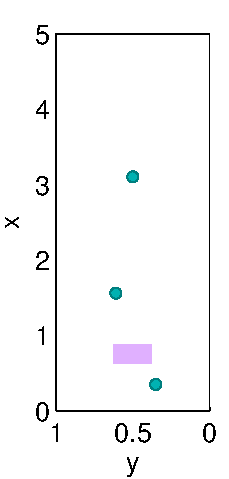
\includegraphics[width=0.8\textwidth]{baseSeries/setup_3_3.pdf}
\caption{Locations of the observations and the QoI region.}
\label{fig:baseSetup}
\end{figure}
%

For the numerical simulations, we use the finite element method (FEM), employing a continuous Galerkin formulation with Lagrange elements. We use the \texttt{libMesh} library~\cite{libMeshPaper} for the FEM calculations. \red{The library offers easy calculation of adjoint systems, error estimates and subdomain restricted variables.}\footnote{But we don't use Libmesh's error estimates or restrict variables to subdomains...} The domain is discretized by a regular mesh of quadrilaterals, with 250 and 50 elements along the $x_1$ and $x_2$ directions, respectively, for a total of 12,500 elements, resulting in 12,801 degrees of freedom per variable. The diffusion coefficient is chosen so that the cell P\'{e}clet number never exceeds 0.1, and thus no stabilization is required.
%
%------------------------------------------------------------%
\subsubsection{Adaptive Model Refinement Results} \label{sec:cdvcdrBaseRef} 
%------------------------------------------------------------%
%
We now present the results for solving the inference problem using Algorithm~\ref{alg:refSeries}. Once the QoI error estimate is calculated using Equation~(\ref{eq:finErrExp}), the error estimate is then decomposed into local contributions, as described in Equation~(\ref{eq:basisblame}). At each iteration, based on this decomposition, we choose the basis functions with the largest error contributions until an additional 5\% of the elements has been marked for refinement. This is repeated until the estimated absolute relative error in the QoI, is less than $1\%$.

Figure~\ref{fig:baseRef} shows the local error contributions, as well as the subdomains where the low- and high-fidelity models are used, for the series of mixed-fidelity models thus generated. Each linear Lagrange basis function's contribution is plotted at its nonzero node.
%
\begin{figure}[h]
\captionsetup[subfigure]{justification=centering,aboveskip=-10pt}
\centering
  \begin{subfigure}[b]{\textwidth}
  \centering    
    \includegraphics[width=0.48\textwidth]{baseSeries/cd_cdr_LF_divvy.png}
    \includegraphics[width=0.51\textwidth]{baseSeries/err_breakdown_LF.png}
    \vspace{-0.5\baselineskip}
    \caption{MF$_0$ ($0\%$ HF)}
    \label{fig:baseRef0}
    \vspace{0.8\baselineskip}
  \end{subfigure}
	\begin{subfigure}[b]{\textwidth}
  \centering
    \includegraphics[width=0.48\textwidth]{baseSeries/cd_cdr_MF01_divvy.png}
    \includegraphics[width=0.51\textwidth]{baseSeries/err_breakdown_MF01.png}
    \vspace{-0.5\baselineskip}
    \caption{MF$_1$ ($5\%$ HF)}
    \vspace{0.8\baselineskip}
  \end{subfigure}
  \begin{subfigure}[b]{\textwidth}
  \centering
    \includegraphics[width=0.48\textwidth]{baseSeries/cd_cdr_MF02_divvy.png}
    \includegraphics[width=0.51\textwidth]{baseSeries/err_breakdown_MF02.png}
    \vspace{-0.5\baselineskip}
    \caption{MF$_2$ ($10\%$ HF)}
    \vspace{0.8\baselineskip}
  \end{subfigure}
\caption{Local error contributions (right) and domain division (left; low-fidelity convection-diffusion model used in red portion, high-fidelity convection-diffusion-reaction model used in blue portion) for mixed-fidelity models.}
\label{fig:baseRef}
\end{figure}
%
Note that the error contribution of each basis function whose support is entirely within the high-fidelity regions is zero.

We see that the largest local error contribution is concentrated in the QoI region, and the data point closest to the QoI. In the first decomposition of the error (Figure~\ref{fig:baseRef0}), the region where the elemental error is maximum is the leftmost data point. Since the constraining model is an elliptic PDE, with a weak convection, information flow is localized, and is weakly convected from left to right. Therefore, for the calculation of the QoI, it is most important to refine the region near the leftmost data point, and the QoI region. After that, the error decomposition suggests refinement in regions upstream and around the middle data point, and then the rightmost data point.

Figure~\ref{fig:baseErr} shows the true and estimated absolute relative errors in the QoI for the various mixed-fidelity models generated by Algorithm~\ref{alg:refSeries}. In this case, we see that the QoI error of only $1\%$ is attained with a mixed-fidelity model where the high-fidelity model is used in only about $10\%$ of the domain. We note that, in general, there is no guarantee that either the error in the QoI or the relative error in the error estimate will decrease monotonically as more of the domain is refined.
%
\begin{figure}[h]
\centering
\includegraphics[width=0.8\textwidth]{baseSeries/err_est.pdf}
\caption{True and estimated absolute relative error in QoI, plotted as a function of the percentage area of the domain in which the high-fidelity convection-diffusion-reaction model is used.}
\label{fig:baseErr}
\end{figure}
%

%------------------------------------------------------------%
\subsubsection{Interaction of Observations and QoI} \label{sec:qoivdata}
%------------------------------------------------------------%
%
The error estimate decomposition (\ref{eq:basisblame}) suggests the use of the high-fidelity model in areas of the domain that are important to the interaction of the observations and QoI; the interaction of these two can be complex, and the areas suggested for refinement may be nonintuitive. To see this, we compare the error estimate decomposition for three sizes of the QoI region $\Omega_I$ given the same set of data points, and for three nested sets of data points given the same QoI region. For the sake of illustration, we make two refinement iterations for each combination of observations and QoI region, regardless of the magnitude of the relative error estimate. However, it was noticed that the number of iterations needed to achieve a given tolerance increased as the QoI region increased, but did not consistently increase or decrease with the number of data points.

The error decomposition for three increasingly large, nested QoI regions $\Omega_I$ given the same set of observations is shown in Figure \ref{fig:qoiStudy}. The bottom row gives the baseline case presented in Section~\ref{sec:cdvcdrBaseRef}, although here we choose the basis functions $i$ whose error $\varepsilon_i$ are among the largest $5\%$, so the proportion of additional refined elements in each iteration is slightly larger. Although refinement is still most important around the data point closest to $x_1=0$, as the QoI region expands the other two data points become more important in that the error decomposition suggests refinement around them earlier. As the QoI region expands, it is also more clearly noticeable that refinement is not equally important in all parts of the QoI region.

\begin{figure}[h]
\captionsetup[subfigure]{justification=centering}
\centering
  \begin{subfigure}[t]{0.20\textwidth}
  \centering
    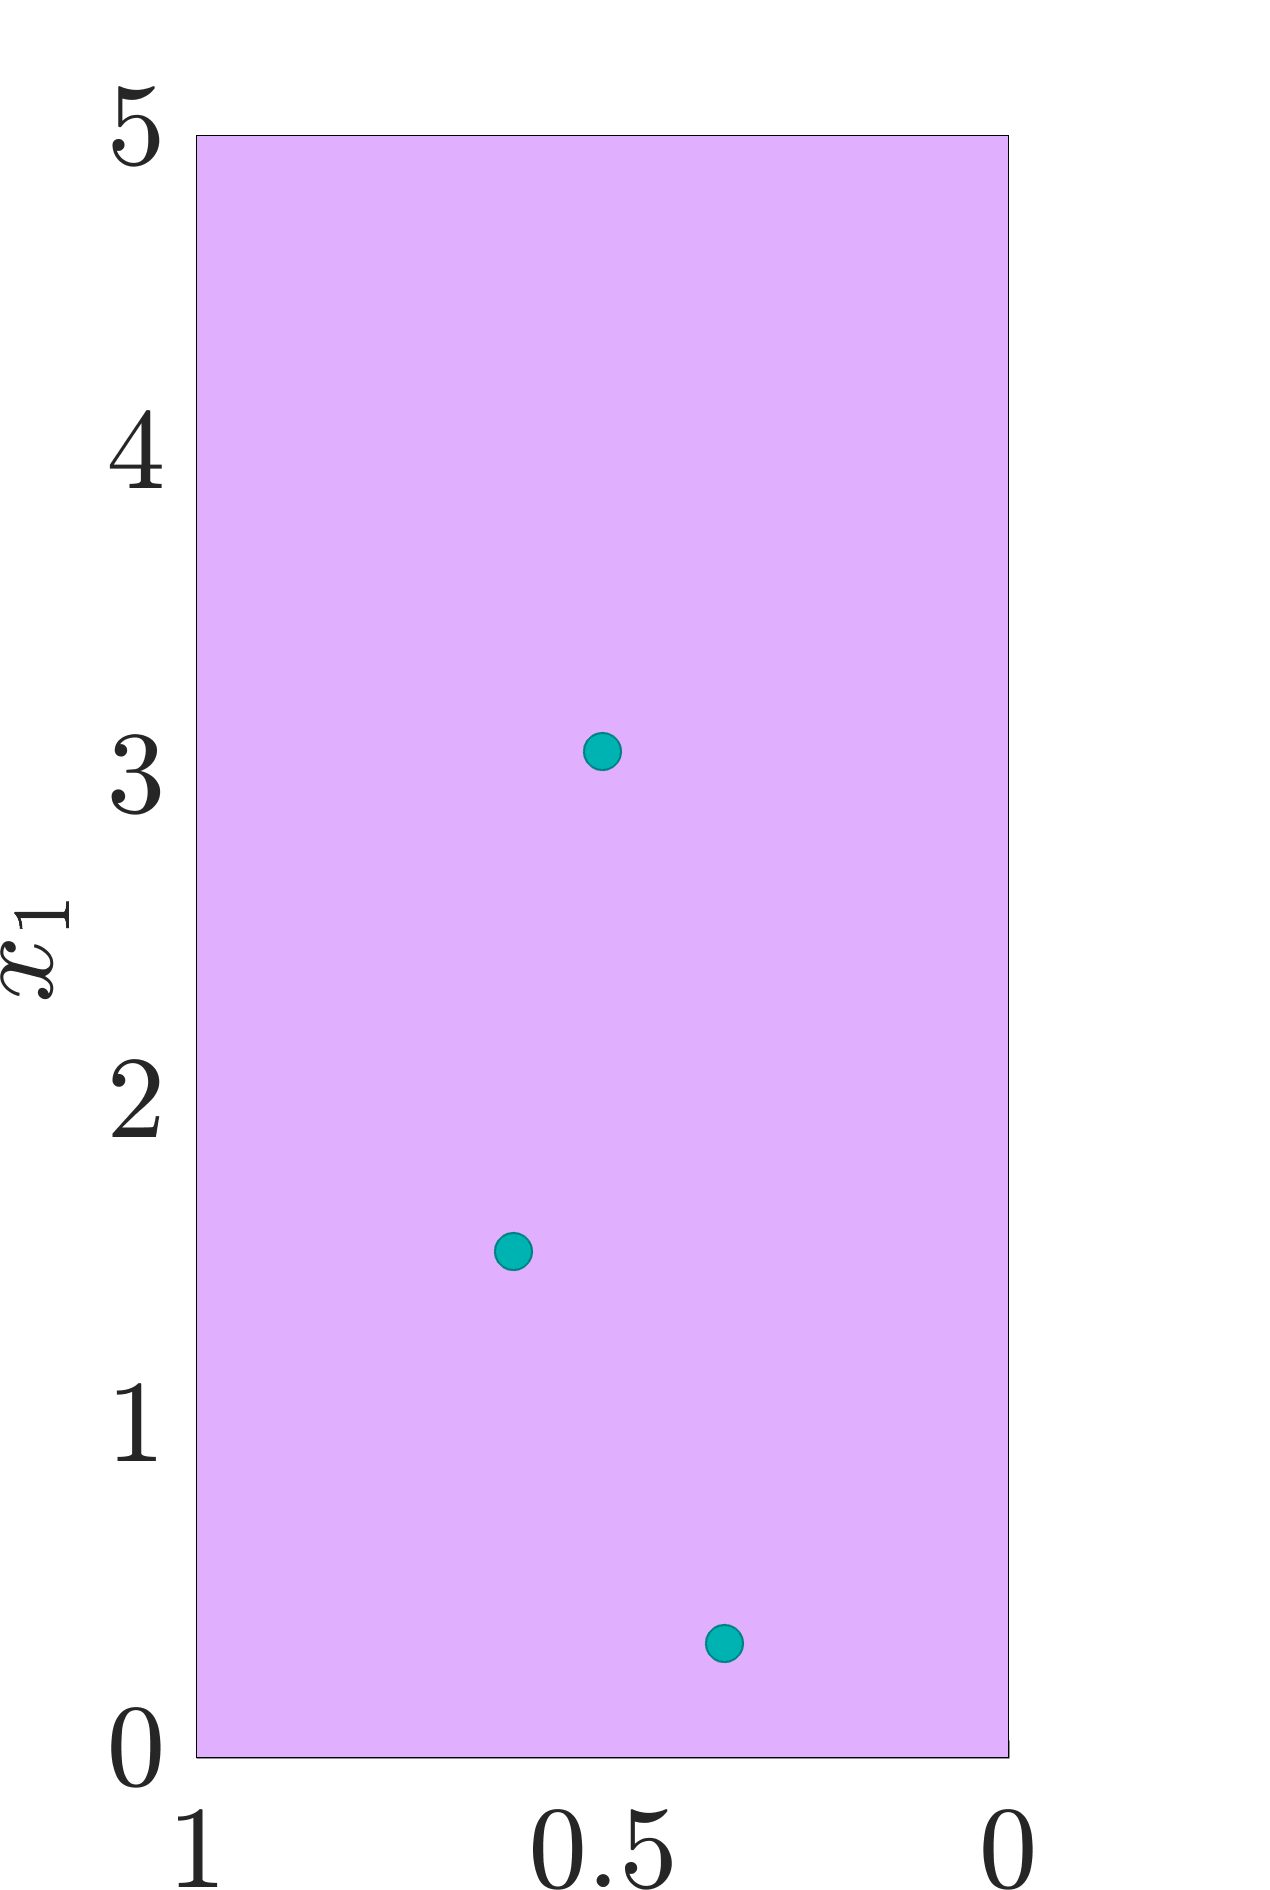
\includegraphics[width=\textwidth]{vs_qoi/qoi5_sens3/setup_5_3.png}
    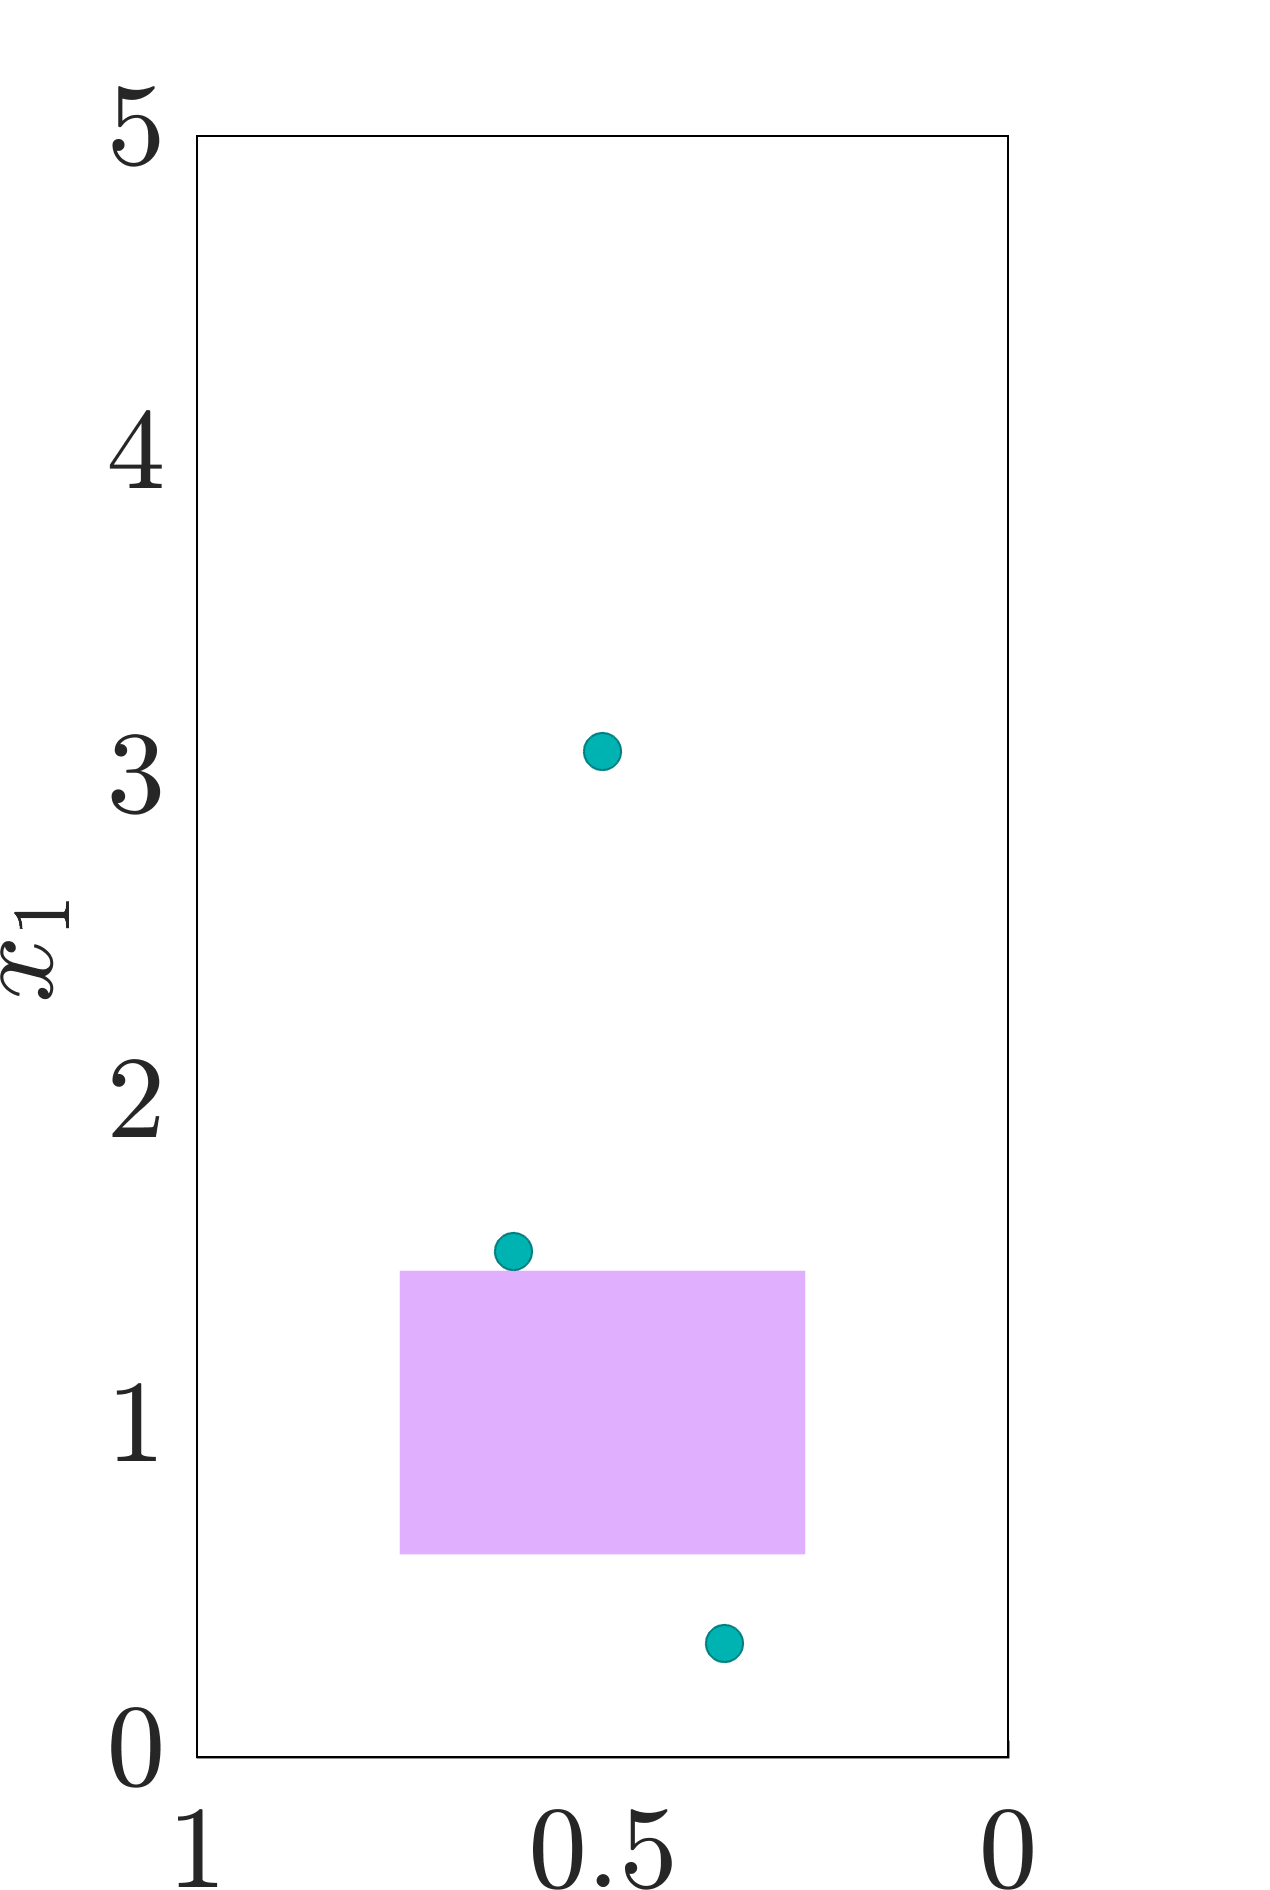
\includegraphics[width=\textwidth]{vs_qoi/qoi7_sens3/setup_7_3.png}
    \includegraphics[width=\textwidth]{vs_qoi/qoi3_sens3/setup_3_3.png}
    \caption{Locations of observations and QoI region $\Omega_I$}
    \label{subfig:obsSetup}
  \end{subfigure}
  \begin{subfigure}[t]{0.20\textwidth}
  \centering
    \includegraphics[width=\textwidth]{vs_qoi/qoi5_sens3/err_breakdown_0.png}
    \includegraphics[width=\textwidth]{vs_qoi/qoi7_sens3/err_breakdown_0.png}
    \includegraphics[width=\textwidth]{vs_qoi/qoi3_sens3/err_breakdown_0.png}
    \caption{MF$_0$ \\ ($0\%$ HF)}
    \label{subfig:obsLF}
  \end{subfigure}
  \begin{subfigure}[t]{0.20\textwidth}
  \centering
    \includegraphics[width=\textwidth]{vs_qoi/qoi5_sens3/err_breakdown_1.png}
    \includegraphics[width=\textwidth]{vs_qoi/qoi7_sens3/err_breakdown_1.png}
    \includegraphics[width=\textwidth]{vs_qoi/qoi3_sens3/err_breakdown_1.png}
    \caption{MF$_1$ \\ ($\sim5\%$ HF)}
  \end{subfigure}
  \begin{subfigure}[t]{0.20\textwidth}
  \centering
    \includegraphics[width=\textwidth]{vs_qoi/qoi5_sens3/err_breakdown_2.png}
    \includegraphics[width=\textwidth]{vs_qoi/qoi7_sens3/err_breakdown_2.png}
    \includegraphics[width=\textwidth]{vs_qoi/qoi3_sens3/err_breakdown_2.png}
    \caption{MF$_2$ \\ ($\sim10\%$ HF)}
    \label{subfig:obsMFlast}
  \end{subfigure}
  \caption{Compare the error estimate decomposition (\subref{subfig:obsLF}-\subref{subfig:obsMFlast}), given the same observations (teal points in (\subref{subfig:obsSetup})) and varying QoI region (purple box in (\subref{subfig:obsSetup})).}
  \label{fig:qoiStudy}
\end{figure}

The error decomposition for three increasing, nested sets of observations and the same QoI region $\Omega_I$ is shown in Figure \ref{fig:dataStudy}. Again, the bottom row gives the baseline case presented in Section~\ref{sec:cdvcdrBaseRef}, although here the basis functions with the largest $5\%$ of the error are chosen, so the proportion of additional refined elements in each iteration is slightly larger. Refinement appears to be consistently most important around the data point closest to $x_1=0$ and the QoI region. However, as more data points are added, it becomes no longer necessarily true that refinement becomes less important around data points as their distance from the QoI region increases. The data points also interact with each other in that placing data points in regions of previously relatively uniform error contribution tends to result in a new error decomposition that is positive or negative around the data points, with valleys of zero magnitude in between.

\begin{figure}[h]
\captionsetup[subfigure]{justification=centering}
\centering
  \begin{subfigure}[t]{0.20\textwidth}
  \centering
    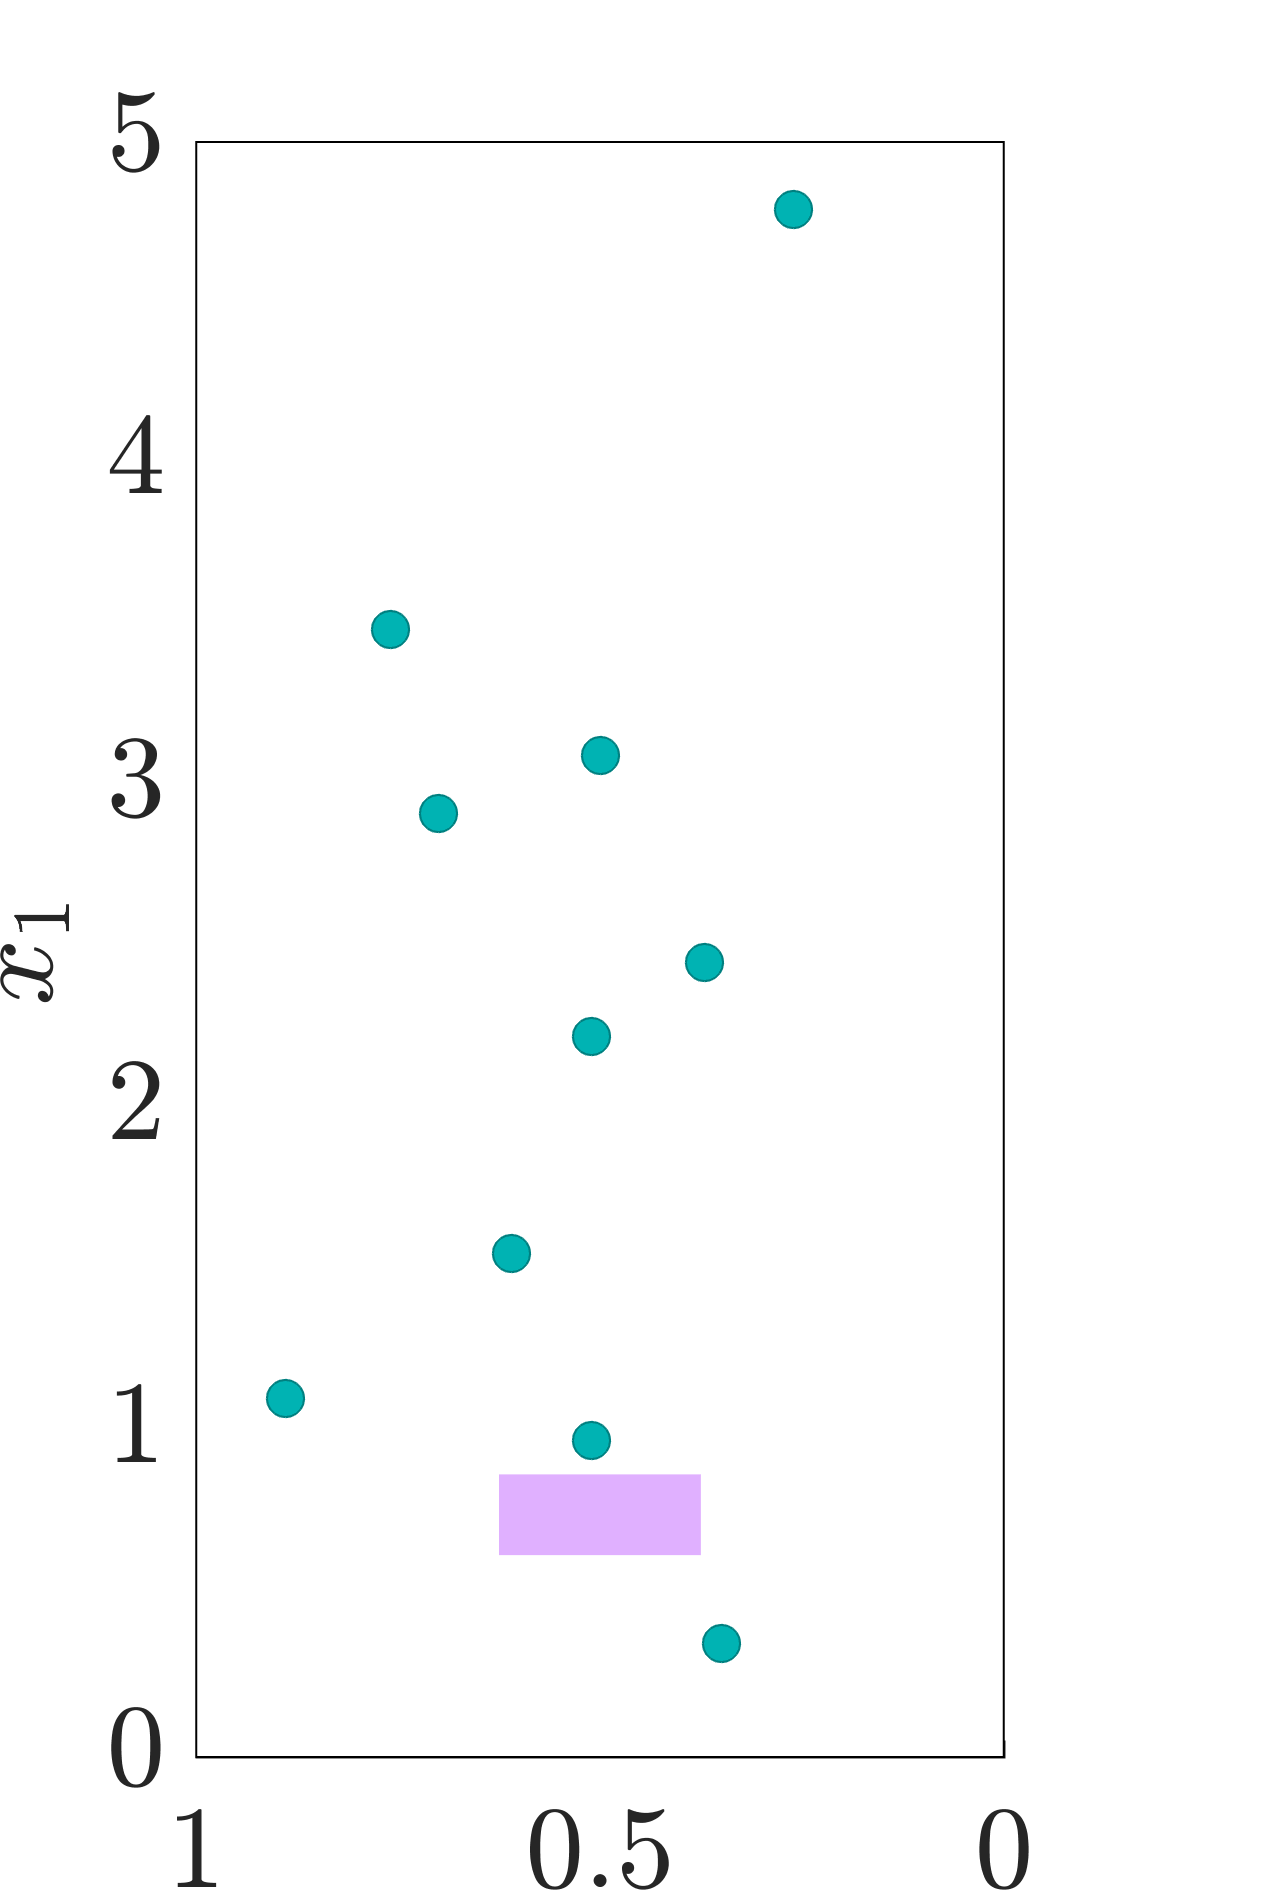
\includegraphics[width=\textwidth]{vs_data/qoi3_sens10/setup_3_10.png}
    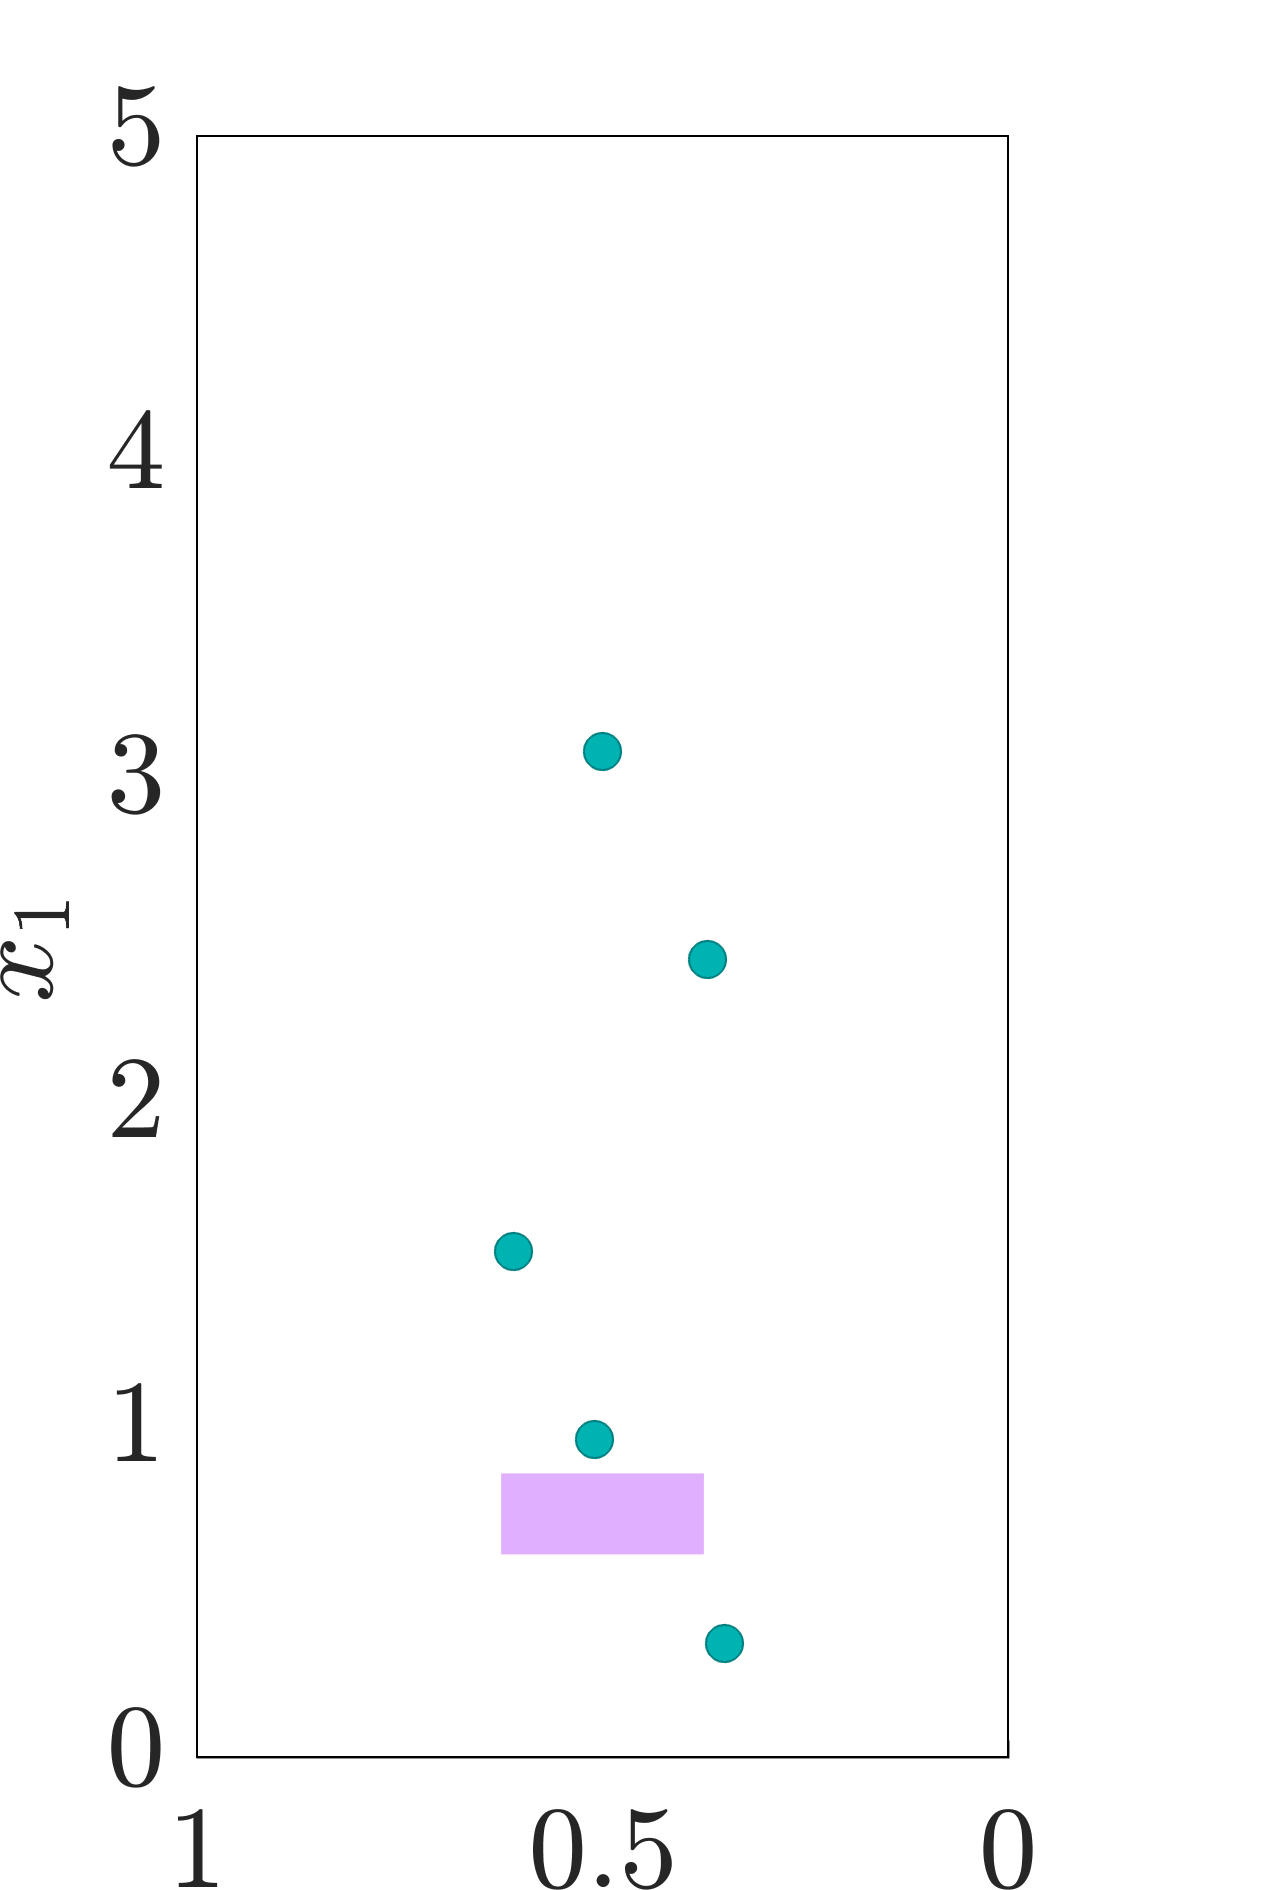
\includegraphics[width=\textwidth]{vs_data/qoi3_sens5/setup_3_5.png}
    \includegraphics[width=\textwidth]{vs_data/qoi3_sens3/setup_3_3.png}
    \caption{Locations of observations and QoI region $\Omega_I$}
    \label{subfig:obsSetup2}
  \end{subfigure}
  \begin{subfigure}[t]{0.20\textwidth}
  \centering
    \includegraphics[width=\textwidth]{vs_data/qoi3_sens10/err_breakdown_0.png}
    \includegraphics[width=\textwidth]{vs_data/qoi3_sens5/err_breakdown_0.png}
    \includegraphics[width=\textwidth]{vs_data/qoi3_sens3/err_breakdown_0.png}
    \caption{MF$_0$ \\ ($0\%$ HF)}
    \label{subfig:obsLF2}
  \end{subfigure}
  \begin{subfigure}[t]{0.20\textwidth}
  \centering
    \includegraphics[width=\textwidth]{vs_data/qoi3_sens10/err_breakdown_1.png}
    \includegraphics[width=\textwidth]{vs_data/qoi3_sens5/err_breakdown_1.png}
    \includegraphics[width=\textwidth]{vs_data/qoi3_sens3/err_breakdown_1.png}
    \caption{MF$_1$ \\ ($\sim5\%$ HF)}
  \end{subfigure}
  \begin{subfigure}[t]{0.20\textwidth}
  \centering
    \includegraphics[width=\textwidth]{vs_data/qoi3_sens10/err_breakdown_2.png}
    \includegraphics[width=\textwidth]{vs_data/qoi3_sens5/err_breakdown_2.png}
    \includegraphics[width=\textwidth]{vs_data/qoi3_sens3/err_breakdown_2.png}
    \caption{MF$_2$ \\ ($\sim10\%$ HF)}
    \label{subfig:obsMFlast2}
  \end{subfigure}
  \caption{Compare the error estimate decomposition (\subref{subfig:obsLF2}-\subref{subfig:obsMFlast2}), given the same QoI region (purple box in (\subref{subfig:obsSetup2})) and varying observations (teal points in (\subref{subfig:obsSetup2})).}
  \label{fig:dataStudy}
\end{figure}

%------------------------------------------------------------------------------------------------------------------------%
\subsection{Constant vs Field Parameters} \label{sec:constvfield}
%------------------------------------------------------------------------------------------------------------------------%
It is not necessary for the low- and high-fidelity models to differ in the physics included. A low-fidelity model may be more computationally tractable due to a reduced number of degrees of freedom rather than reduced nonlinearity. In this section, we consider two models which differ in the space to which the parameter belongs, with the low-fidelity model having fewer degrees of freedom.
%------------------------------------------------------------%
\subsubsection{Problem Setup}
%------------------------------------------------------------%
We consider the same high-fidelity model as in Section~\ref{sec:cdvcdr}:
\begin{equation}
k_d\nabla^2 u - \vec{V}\cdot\nabla u + k_ru^2= f(q),\quad q\in U,
\end{equation}
with the same diffusion coefficient $k_d = 0.1$  and reaction coefficient $k_r = -42$. The low-fidelity model
\begin{equation}
k_d\nabla^2 u - \vec{V}\cdot\nabla u + k_ru^2= f(q),\quad q\in\R
\end{equation}
differs from the high-fidelity model only in that the parameter $q$ is a constant instead of a field. Then the intermediate mixed-fidelity models have parameter fields which are non-constant in only portions of the domain. For ease of implementation, we require that the resulting parameter field remain continuous at the interface between the low-fidelity and high-fidelity subdomains, although this constraint is not necessary for the theory to hold. The domain, mesh, boundary conditions, and velocity field, as well as the observations, unknown parameters to be inferred, and QoI, remain the same as described in Section~\ref{sec:cdvcdr}. As the inverse problem is ill-posed, except for perhaps in the case where the low-fidelity model is used throughout the domain, regularization is added; the Tikhonov regularization term is $\frac{\beta}{2}\int_\Omega \|\nabla f(q)\|_2^2+f(q)^2\:\textrm{d}A$, where $\beta=10^{-3}$ is a regularization coefficient.

Although using such a pair of models has similarities to the problem of adaptive mesh refinement, we note that when seeking adaptive mesh refinement for the goal-oriented inverse problem, it is more efficient to use the approach discussed in \cite{BecVex05}.
%------------------------------------------------------------%
\subsubsection{Adaptive Model Refinement Results}
%------------------------------------------------------------%
As with the previous examples in Section~\ref{sec:cdvcdr}, the decomposition (\ref{eq:basisblame}) of the error estimate is used to select additional regions of the domain in which to use the high-fidelity model. The number of degrees of freedom in the inverse problem increases with the proportion of the domain in which the high-fidelity model is used and the unknown parameter allowed to be a field. With each iteration, an additional $10\%$ of the elements are marked for refinement. This is repeated until the estimated absolute relative error in the QoI, is less than $1\%$.

Figure~\ref{fig:svfRef} shows the local error contributions, as well as the subdomains where the low- and high-fidelity models are used, for the first two and last mixed-fidelity model thus generated. Each linear Langrange basis function's contribution is plotted at its nonzero node. 
%
\begin{figure}[h]
\captionsetup[subfigure]{justification=centering,aboveskip=-10pt}
\centering
\begin{subfigure}[b]{\textwidth}
\centering
	\includegraphics[width=0.48\textwidth]{svf/cd_cdr_LF_divvy.png}
  \includegraphics[width=0.51\textwidth]{svf/err_breakdown_LF.png}
  \vspace{-0.7\baselineskip}
  \caption{MF$_0$ ($0\%$ HF)}
  \vspace{0.8\baselineskip}
\end{subfigure}
\begin{subfigure}[b]{\textwidth}
	\centering
	\includegraphics[width=0.48\textwidth]{svf/cd_cdr_MF01_divvy.png}
  \includegraphics[width=0.51\textwidth]{svf/err_breakdown_MF01.png}
  \vspace{-0.7\baselineskip}
  \caption{MF$_1$ ($10\%$ HF)}
  \vspace{0.8\baselineskip}
\end{subfigure}
\begin{subfigure}[b]{\textwidth}
  \centering
  \includegraphics[width=0.48\textwidth]{svf/cd_cdr_MF02_divvy.png}
  \includegraphics[width=0.51\textwidth]{svf/err_breakdown_MF02.png}
  \vspace{-0.7\baselineskip}
  \caption{MF$_2$ ($20\%$ HF)}
  \vspace{0.8\baselineskip}
\end{subfigure}
%\begin{subfigure}[b]{\textwidth}
%	\centering
%	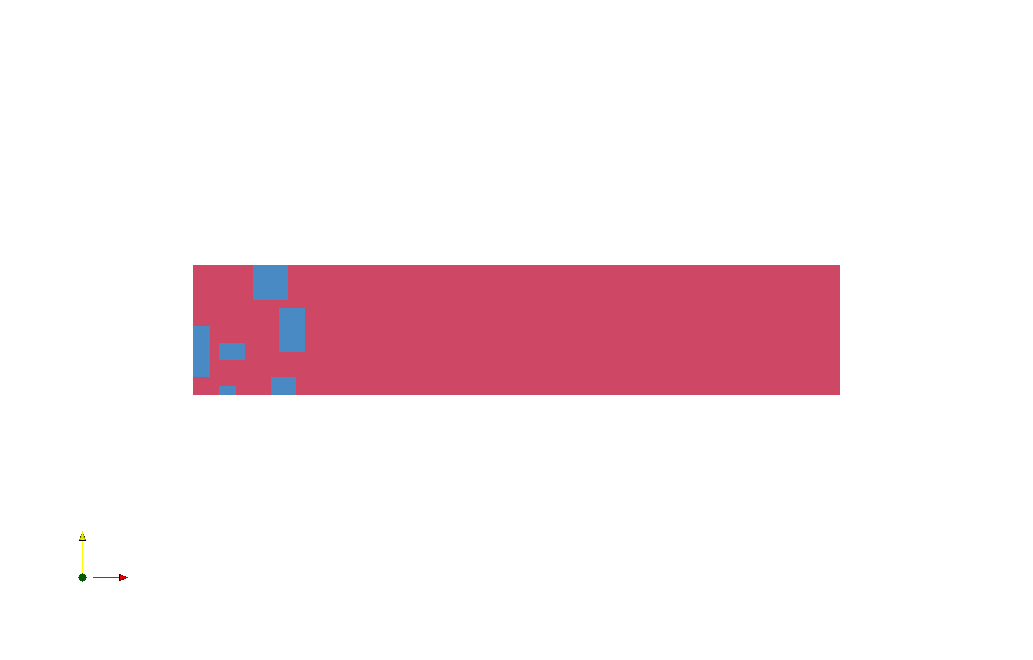
\includegraphics[width=0.48\textwidth]{svf/cd_cdr_MF03_divvy.png}
%  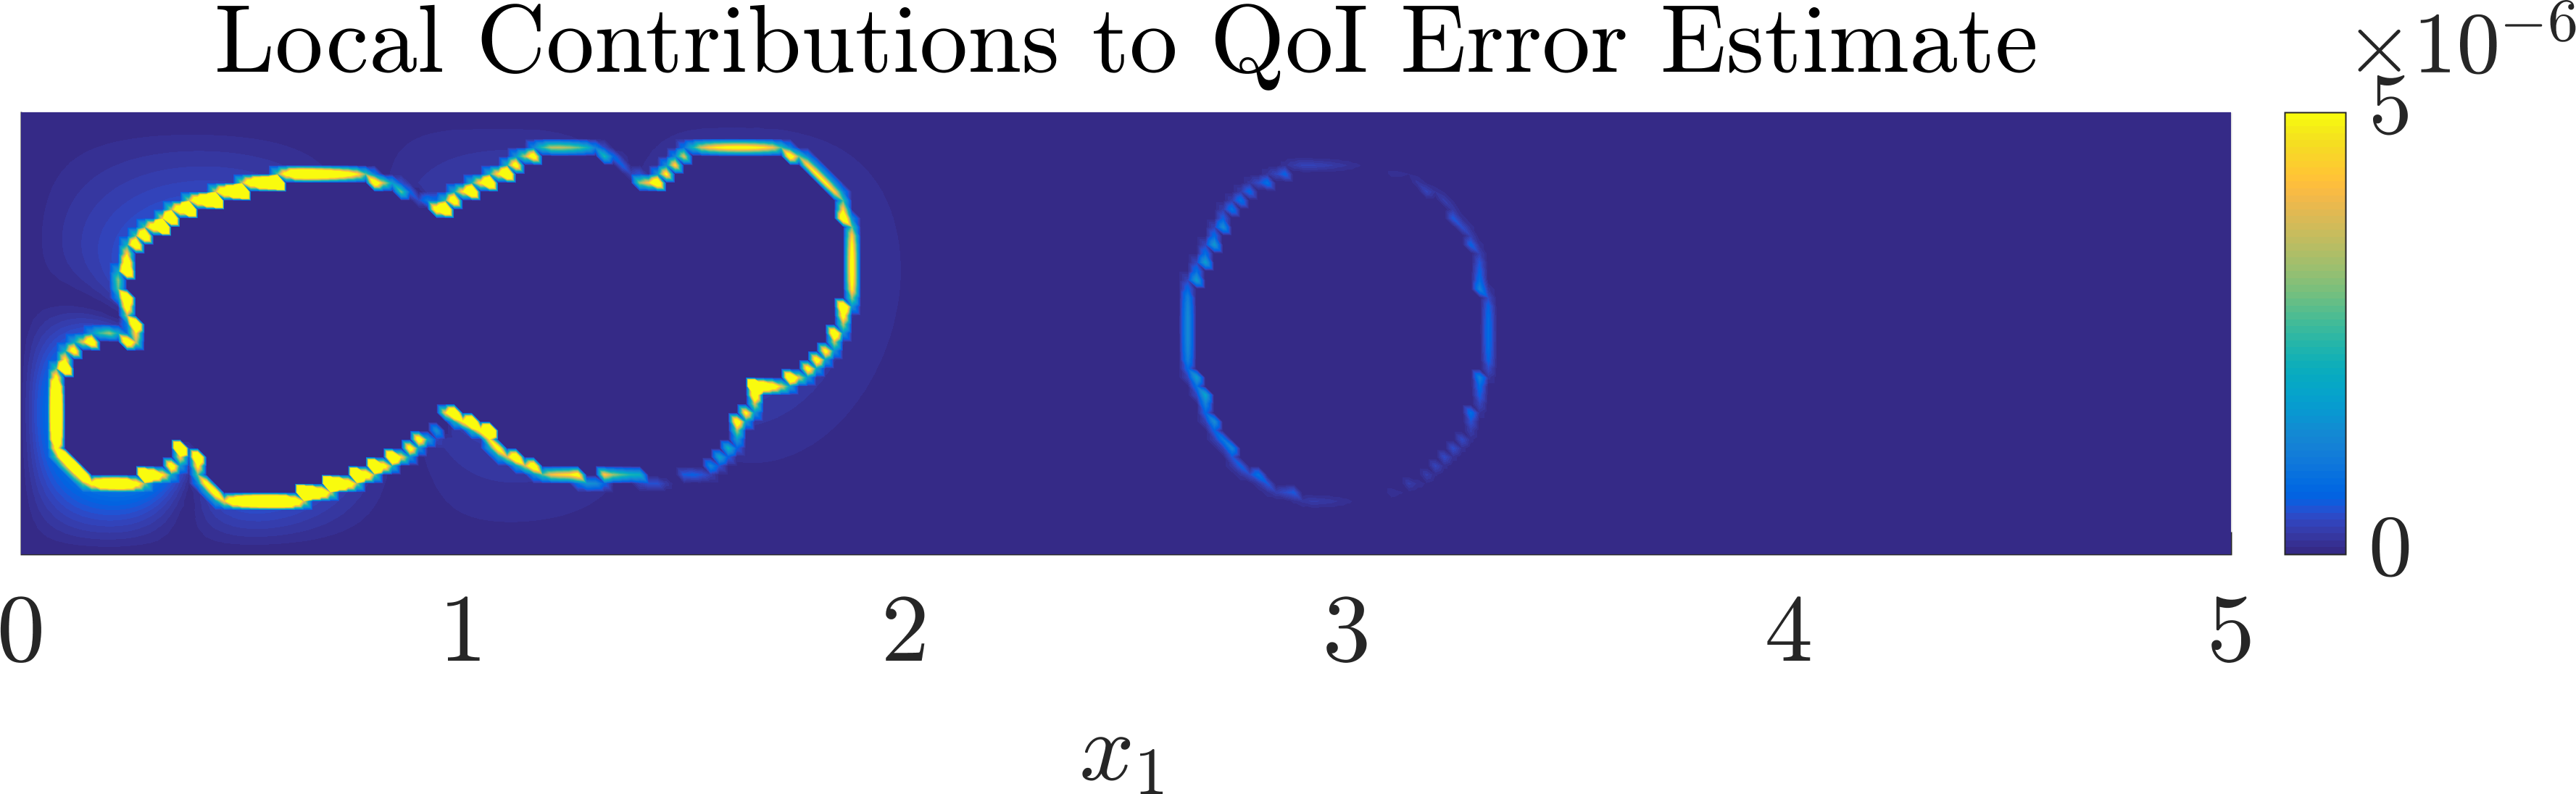
\includegraphics[width=0.51\textwidth]{svf/err_breakdown_MF03.png}
%  \vspace{-0.7\baselineskip}
%  \caption{MF$_3$ ($30\%$ HF)}
%  \vspace{0.8\baselineskip}
%\end{subfigure}
%\begin{subfigure}[b]{\textwidth}
%	\centering
%	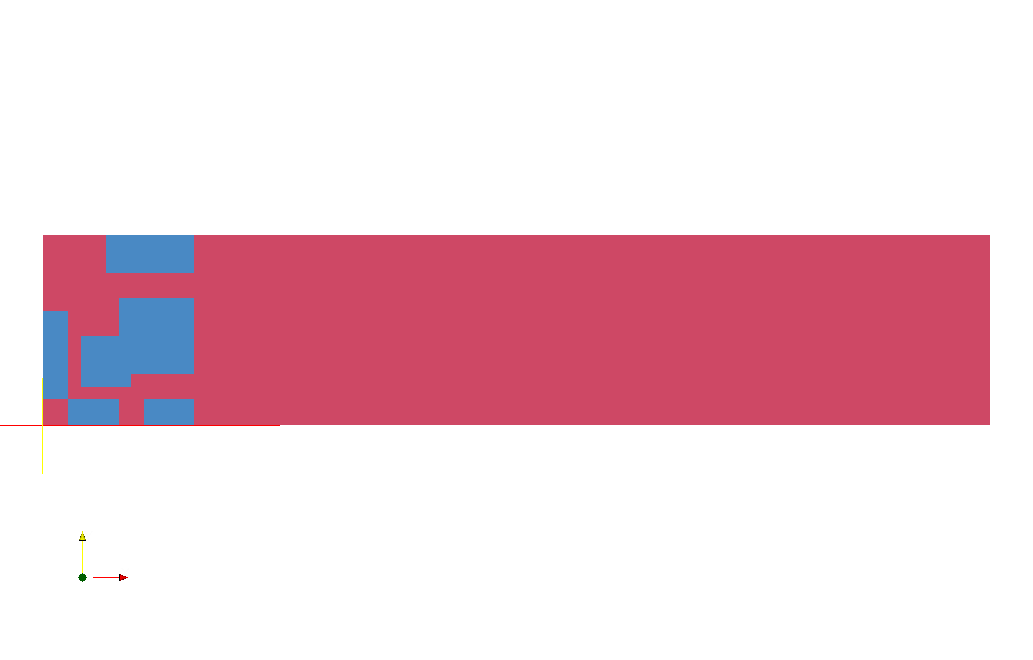
\includegraphics[width=0.48\textwidth]{svf/cd_cdr_MF04_divvy.png}
%  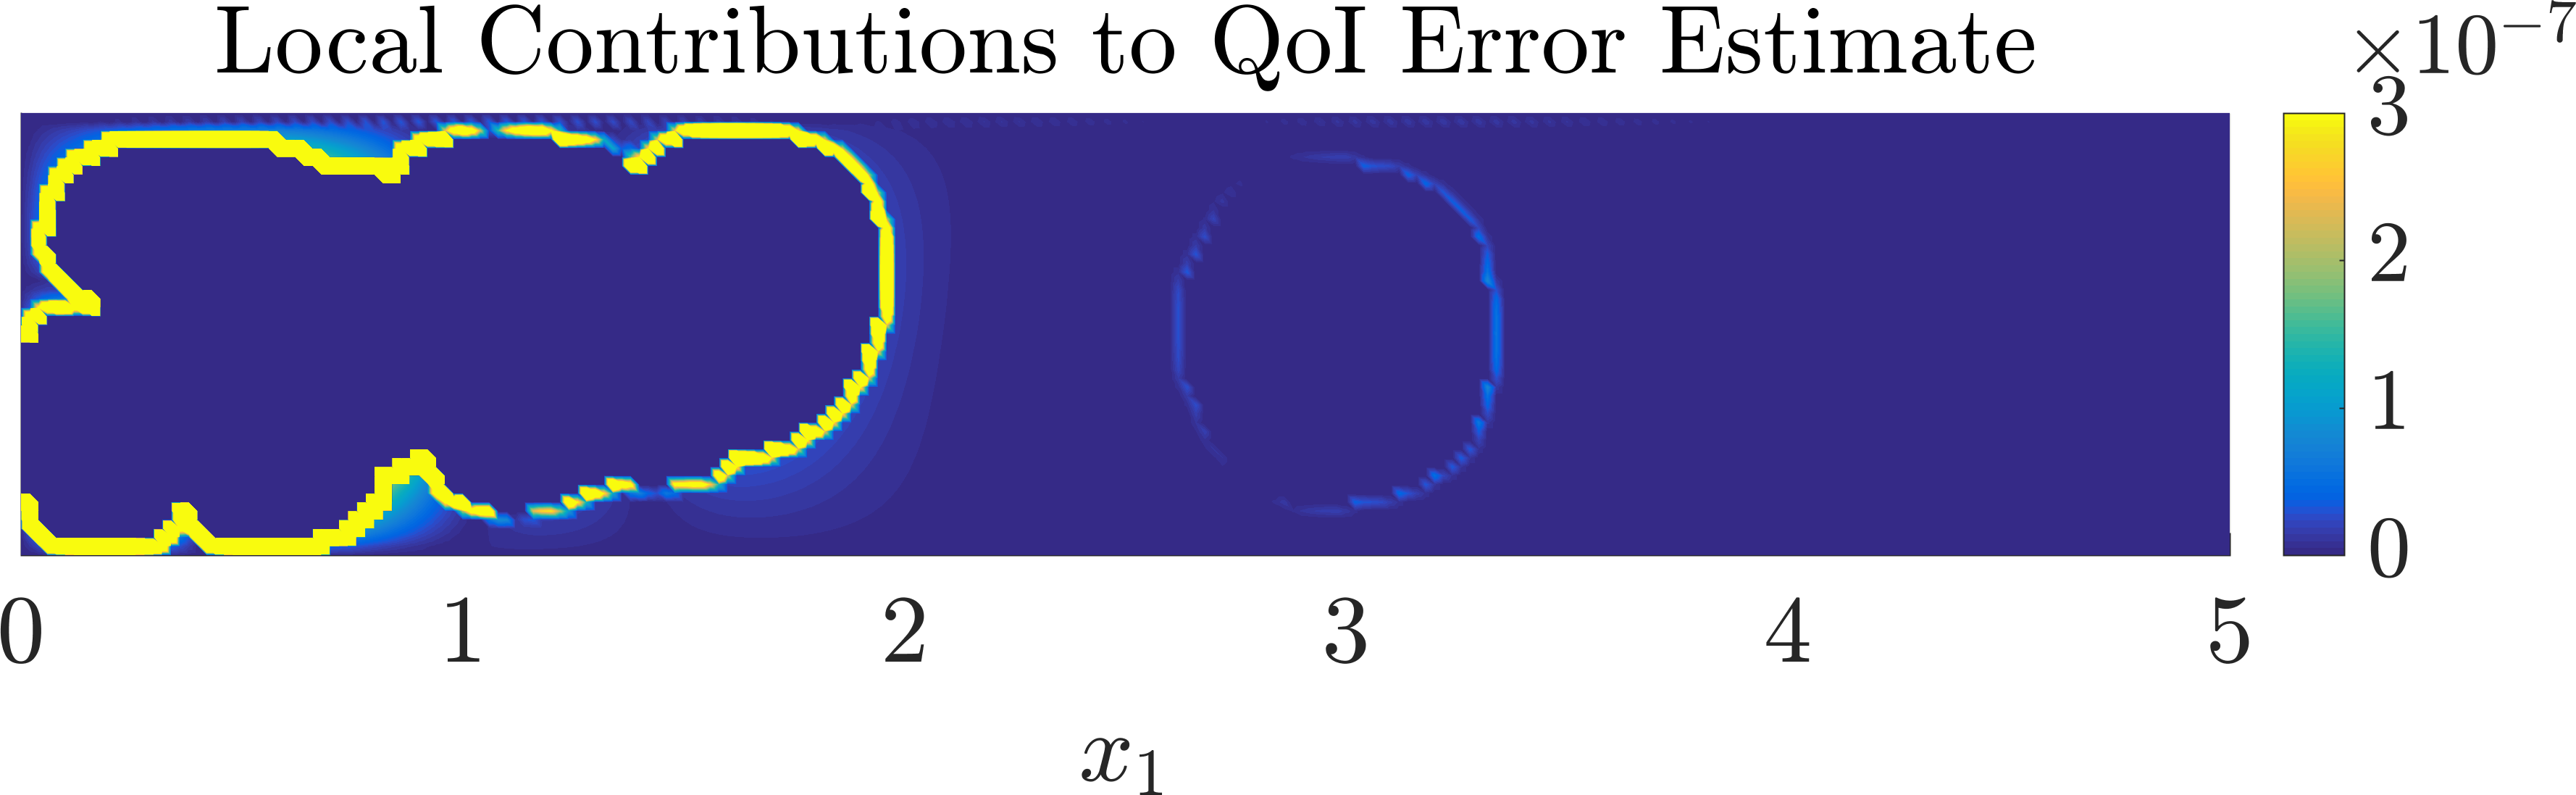
\includegraphics[width=0.51\textwidth]{svf/err_breakdown_MF04.png}
%  \vspace{-0.7\baselineskip}
%  \caption{MF$_4$ ($40\%$ HF)}
%  \vspace{0.8\baselineskip}
%\end{subfigure}
%\begin{subfigure}[b]{\textwidth}
%	\centering
%	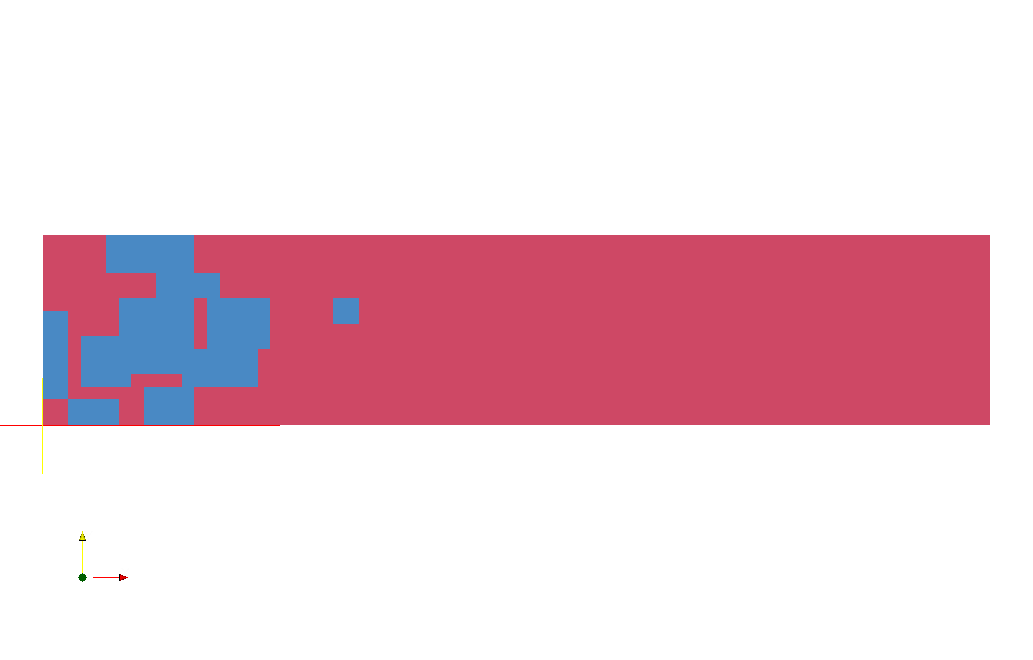
\includegraphics[width=0.48\textwidth]{svf/cd_cdr_MF05_divvy.png}
%  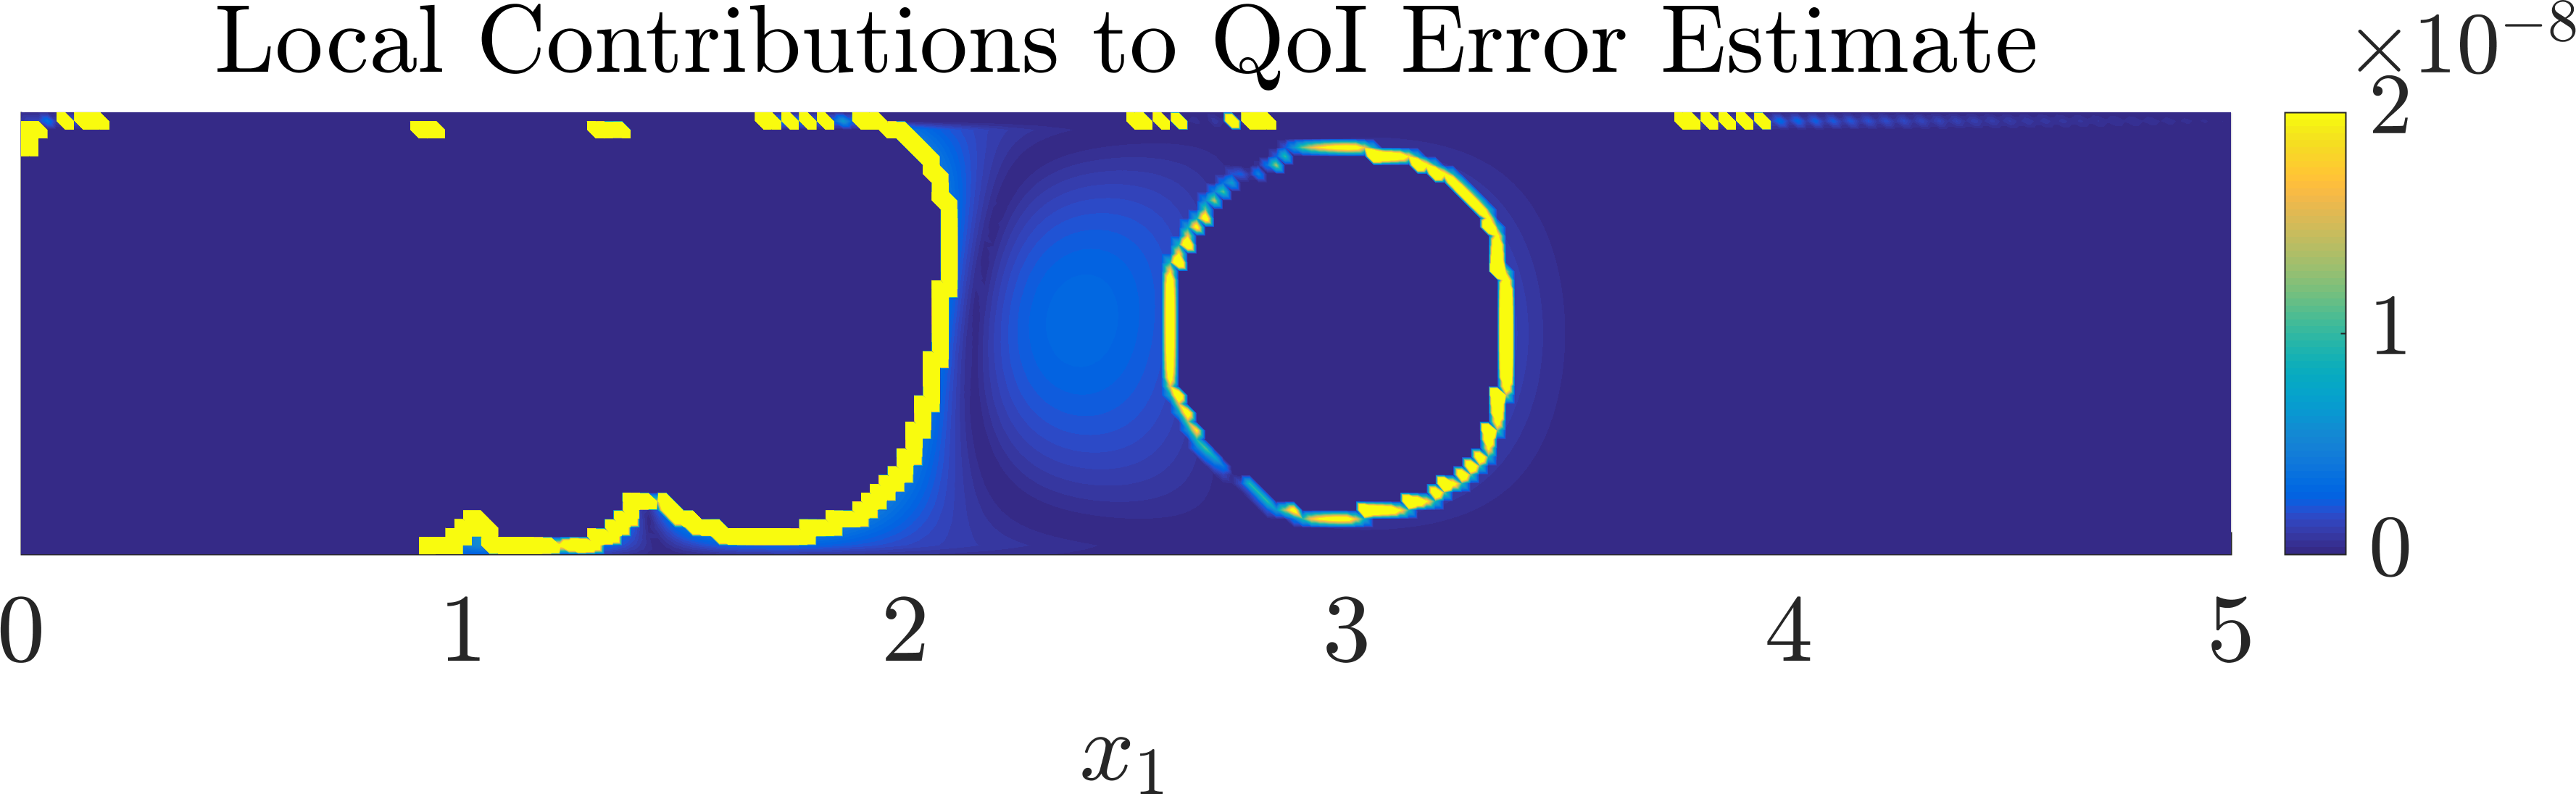
\includegraphics[width=0.51\textwidth]{svf/err_breakdown_MF05.png}
%  \vspace{-0.7\baselineskip}
%  \caption{MF$_5$ ($50\%$ HF)}
%  \vspace{0.8\baselineskip}
%\end{subfigure}
\begin{subfigure}[b]{\textwidth}
	\centering
	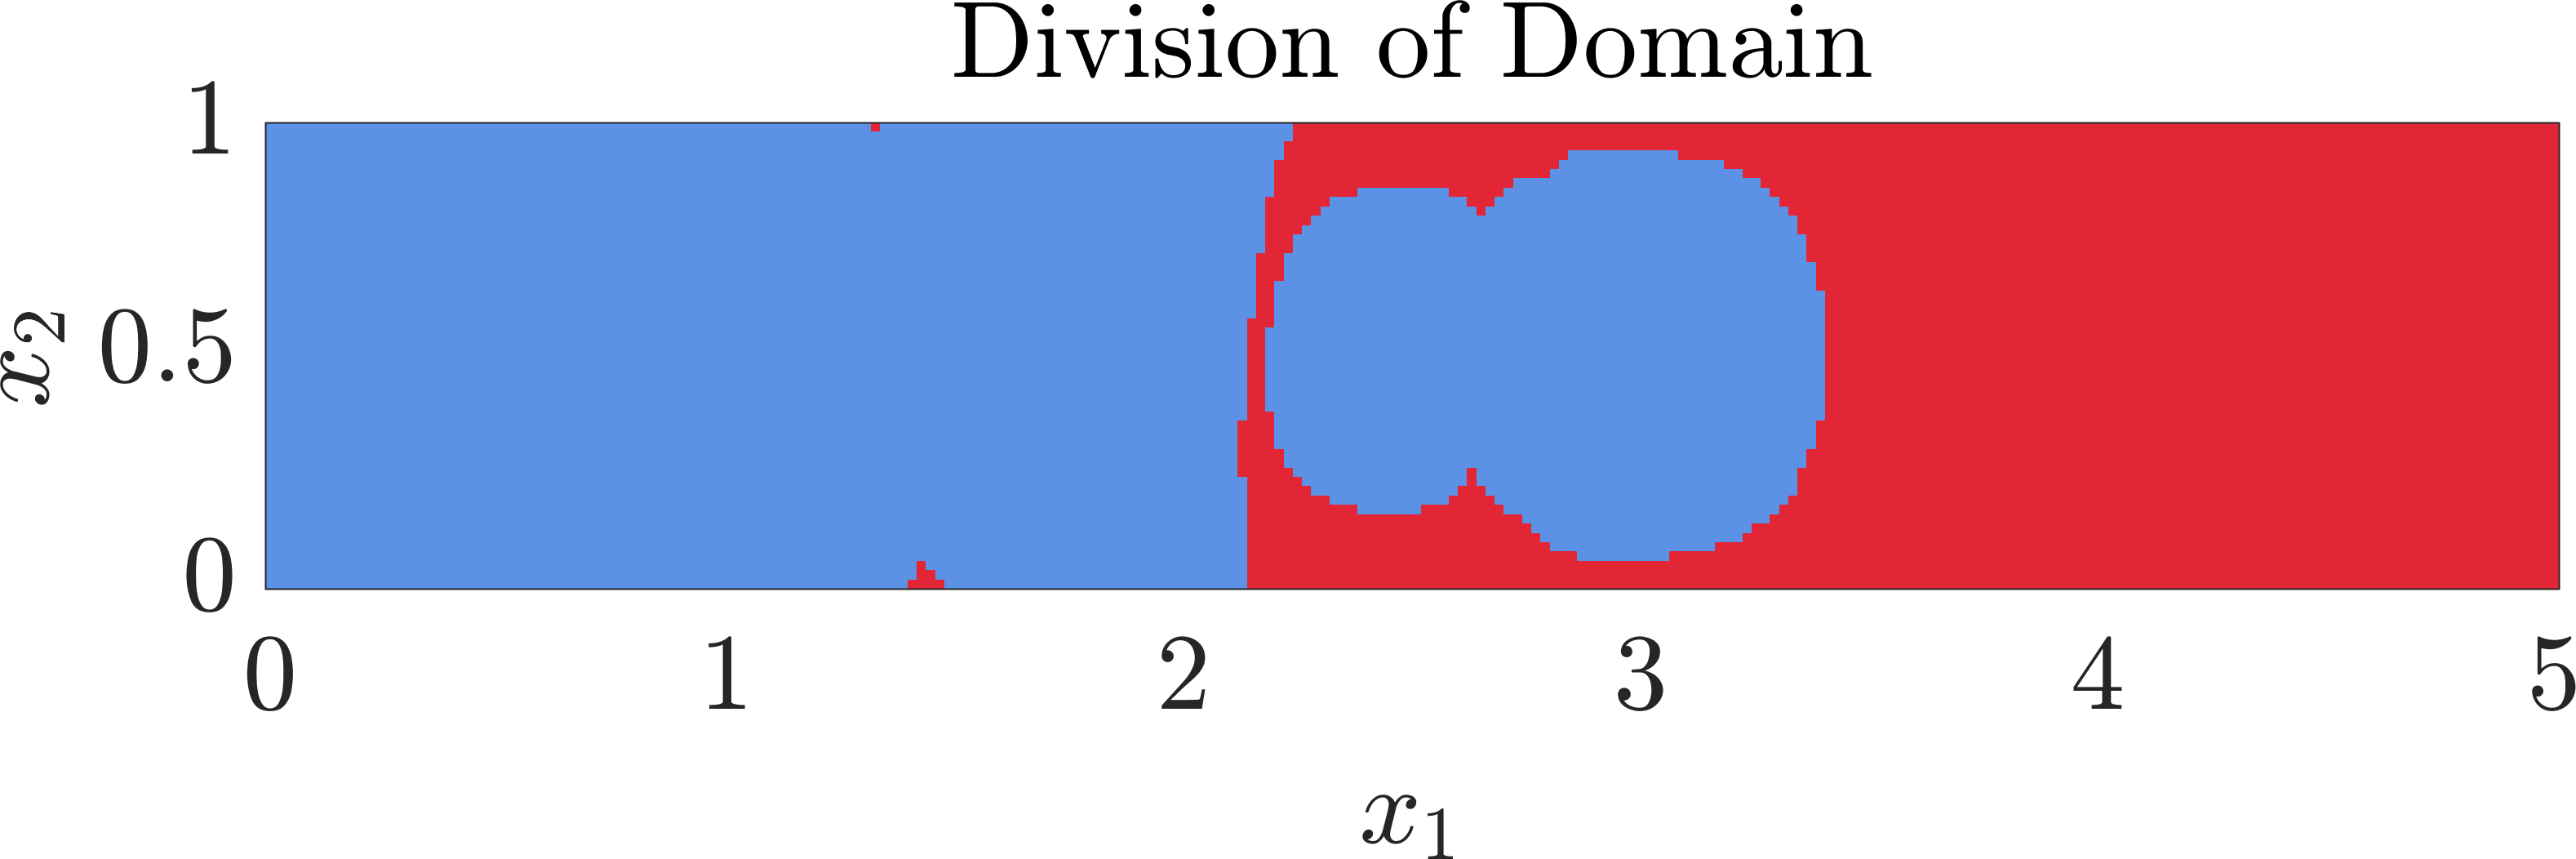
\includegraphics[width=0.48\textwidth]{svf/cd_cdr_MF06_divvy.png}
  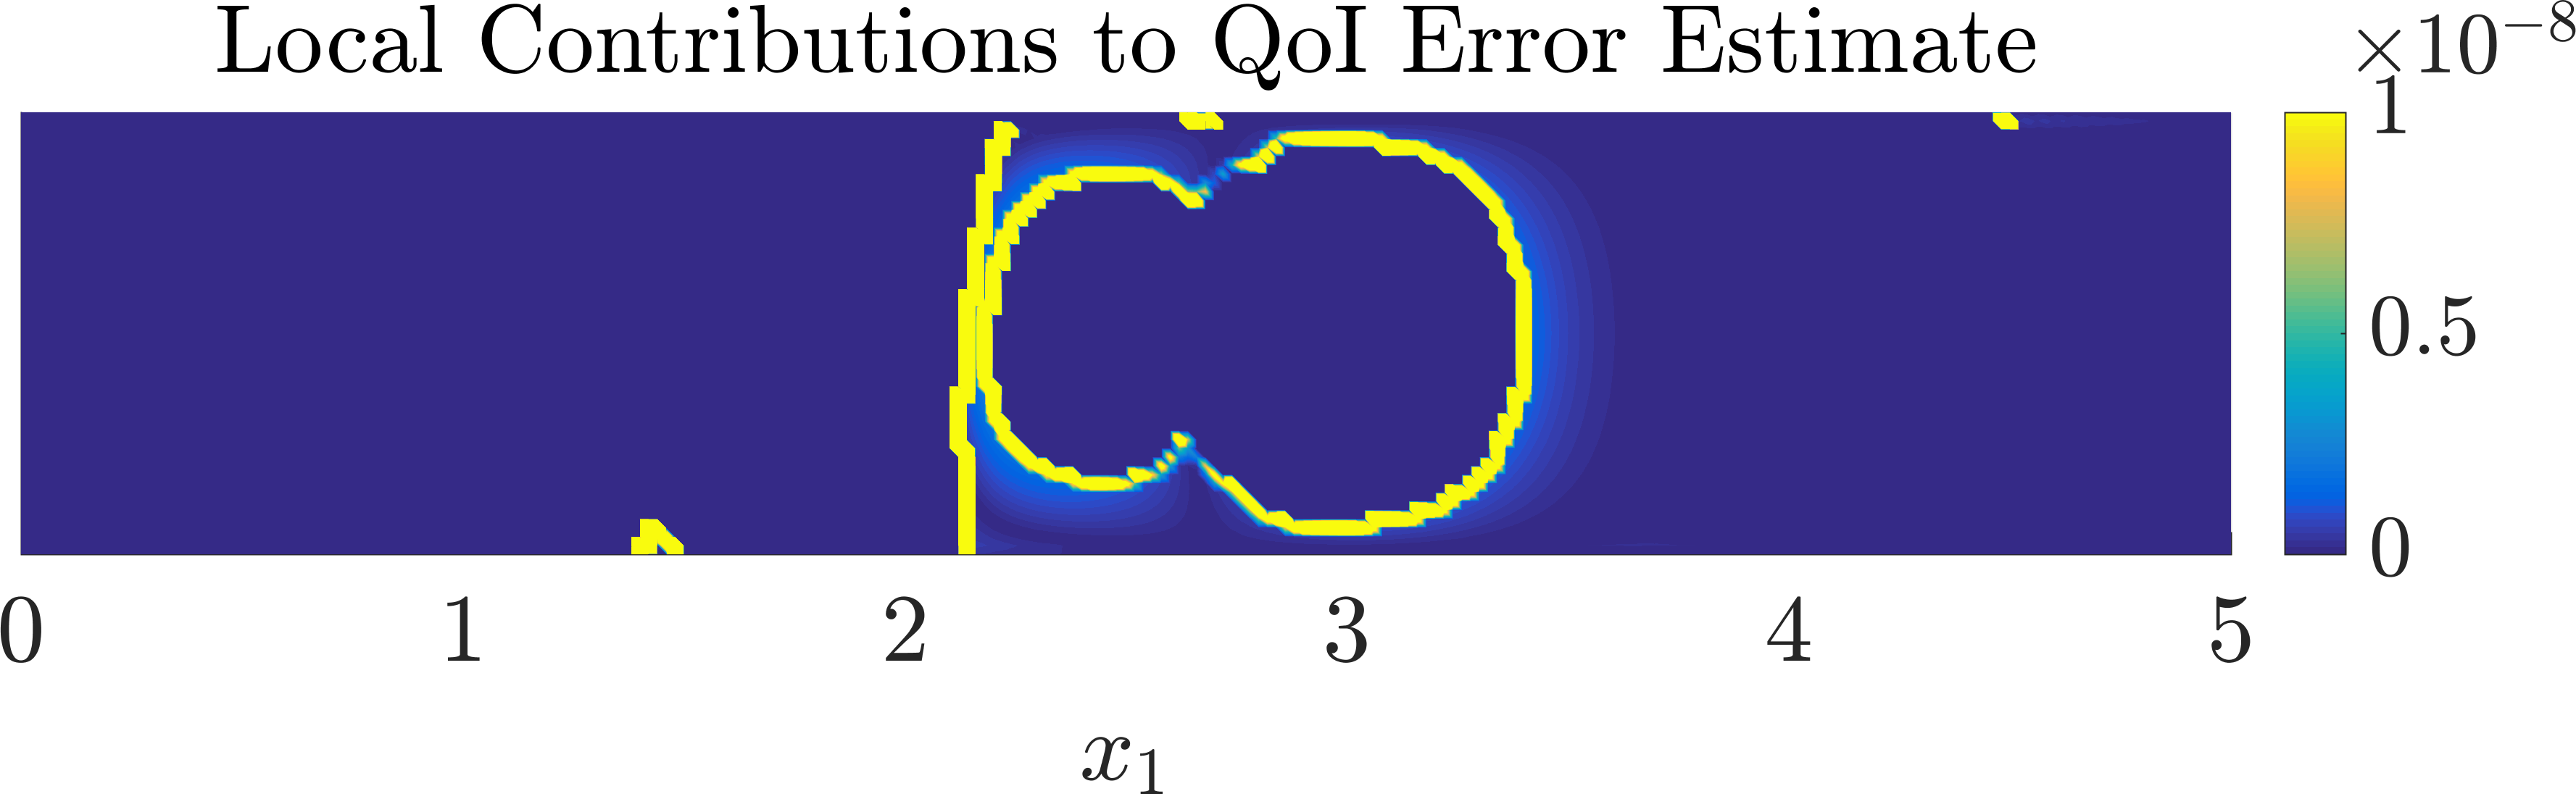
\includegraphics[width=0.51\textwidth]{svf/err_breakdown_MF06.png}
  \vspace{-0.7\baselineskip}
  \caption{MF$_6$ ($60\%$ HF)}
\end{subfigure}
\caption{Local error contributions (right) and domain division (left; low-fidelity constant-parameter model used in red portion, high-fidelity field-parameter model used in blue portion) for mixed-fidelity models. The (weighted) residual, and thus the local error contribution, tends to spike sharply at the interface between the low- and high-fidelity regions; the color range is truncated to make the error distribution visible elsewhere in the domain.}
\label{fig:svfRef}
\end{figure}
%
Comparing to Figure~\ref{fig:baseRef}, we see that in this case the local error contribution is not as greatly concentrated around the QoI region and the nearest data point; here, all three data points and the QoI region have associated regions of sufficiently similar high local error that all are refined in the first iteration. This reflects the global nature of the differences between the low- and high-fidelity models; the parameter field in all the low-fidelity regions is constant and equal. 

The corresponding true and estimated absolute errors in the QoI are shown in Figure~\ref{fig:svfErr}.
%
\begin{figure}[h]
\centering
\includegraphics[width=0.8\textwidth]{svf/err_est.pdf}
\caption{True and estimated absolute relative error in QoI, plotted as a function of the percentage area of the domain in which the high-fidelity field-parameter model is used.}
\label{fig:svfErr}
\end{figure}
%
In this case, we see that we must use the high-fidelity model in most of the domain in order to get an accurate QoI. The adaptive algorithm requires us to use the field representation of the high-fidelity model in much of the left half of the domain; this reflects the topology of the inferred parameter field in the high-fidelity inverse problem, which is only relatively constant towards the right portion of the domain. We also see that in this case, compared to the example in Section~\ref{sec:cdvcdrBaseRef}, increasing the proportion of the domain in which the high-fidelity model is used does not monotonically decrease the error in the QoI. 
%------------------------------------------------------------------------------------------------------------------------%
\subsection{Convection-Diffusion(-Highly Nonlinear Reaction)}
%------------------------------------------------------------------------------------------------------------------------%
\red{Not sure should even keep this section...if we split the supplementary adjoint solve, then the condition for adaptivity being more efficient doesn't depend on the linear solver...we don't need this section to make a cost argument if we have the 3D example...having this section seems to be overkill/redundant if all we want to say is that 'sometimes we need continuation for the HF inverse problem'...if we want to make a 'robustness' argument, then merge with whatever vikram writes about operator continuation interpretation?
%------------------------------------------------------------%
\subsubsection{Results}
%------------------------------------------------------------%

We consider the convection-diffusion-reaction term described in Section \ref{sec:cdvcdr}, with a reaction term $k_r=-616$ in the high-fidelity model. This reaction term is large enough that the Newton solver will not converge with a zero initial guess. We first solve the inverse problem with the low-fidelity model ($k_r=0$), and then use a simple continuation approach, using the solution at one value of $k_r$ as the initial guess for the next.\footnote{not arclength continuation, which is more difficult to implement, though libMesh appears to have a class for such continuation, which we can use if this seems like a viable direction} We increase the reaction term in increments of $\Delta k_r=100$, and halve the increment each time the step is too large (Newton solver does not converge at the next $k_r$ value). From $k_r=0$ to $k_r=-616$, this results in 9 continuation steps being taken.

%------------------------------------------------------------%
\subsubsection{Computational Complexity}
%------------------------------------------------------------%

We compare the complexity of Algorithm~\ref{alg:refSeries} and the continuation method for the high fidelity problem, in the context of the analysis developed in section~\ref{sect:alg_complexity}. For the high fidelity problem, with  with 9 continuation steps, we have $\sum\limits_{i=1}^{C} K_i=30$. 
 
With Gaussian elimination chosen as the linear solver, this gives us $T < 3$, i.e.\ a budget of 2 adaptive steps. Using Algorithm~\ref{alg:refSeries} with 2 refinement steps, and only $10\%$ of the domain refined to use the high-fidelity model, the estimated relative error is $<1\%$. Indeed, the ratio $\frac{C_{MF}}{C_{HF}}$ was $\frac{24}{30}$, indicating about $20\%$ reduction in computational cost, with the worst case linear solver used. 

In other words, on using Algorithm~\ref{alg:refSeries} for a highly nonlinear problem, even with the worst case linear solver, one can get to $<1\%$ error in the QoI, with a $20\%$ reduction in computational cost, while avoiding any need for continuation to handle nonlinearities. }

%------------------------------------------------------------------------------------------------------------------------%
\subsection{Convection-Diffusion(-Reaction) in 3D} \label{sec:cdvcdr3D}
%------------------------------------------------------------------------------------------------------------------------%

In the previous examples, although the low- and high-fidelity models are sufficiently different to illustrate the behavior of Algorithm~\ref{alg:refSeries}, they are both simple enough and similar enough that using Algorithm~\ref{alg:refSeries} saves little, if any, time. In this section, we consider a more realistic pair of models which differ in the physics included, and demonstrate computational savings when using the adaptive algorithm, while still achieving a small error in the QoI. In Section~\ref{sec:setup3D} we describe the setup of the models and their inverse problems, and in Section~\ref{sec:ref3D} we describe the results of applying Algorithm~\ref{alg:refSeries} to this pair of models.

%------------------------------------------------------------%
\subsubsection{Problem Setup} \label{sec:setup3D}
%------------------------------------------------------------%

The two models share a box domain $\Omega(x_1,x_2,x_3)$ which is $2300$m, $1650$m, and $100$m long in the $x_1$, $x_2$, and $x_3$ directions, respectively. We will refer to the positive and negative directions in $x_1$ as ``east" and ``west", respectively. The high-fidelity model is a single-species convection-diffusion-reaction equation with a nonlinear reaction term, described by
%
\begin{subequations}
\label{eq:cdvcdrHF3D}
\begin{align}
\nabla\cdot(n\vec{V}u - nD\nabla u) + k_ru^2 = f(q) \quad &\text{in } \Omega, \label{eq:HFeq3D}\\
u = 5 \quad &\text{on } \partial \Omega_{west}, \\
\frac{\partial u}{\partial n} = 0 \quad &\text{on }\partial\Omega_{east}, \\
\hat{n}\cdot(n\vec{V}u - nD\nabla u) = 0 \quad &\text{on }\partial\Omega\backslash(\partial\Omega_{east}\cup\partial\Omega_{west}),
\end{align} 
\end{subequations}
%
where the state $u$ is the mass-fraction (in parts-per-billion) of some contaminant species and $f(q)$ is a source/sink field. The velocity field is a constant $\vec{V}=(2.1,0,0)$ m/day. Given this velocity field and letting the molecular diffusion be negligble, we follow \cite{Vestedetal93} to express the (diagonal) dispersion tensor $D$ as $D_{11}=\alpha_{LH}V_1$, $D_{22}=\alpha_{TH}V_1$, and $D_{33}=\alpha_{TV}V_1$, where $\alpha_{LH}=100$m, $\alpha_{TH}=40$m, and $\alpha_{TV}=4$m are the longitudinal horizontal, transverse horizontal, and transverse vertical dispersivities, respectively; the dispersivity values were drawn from within the range of observed values in various porous media \cite{Davis86}. We have porosity $n=0.1$. The reaction coefficient is $k_r=4.2\cdot10^{-4}$ 1/day, chosen from within the wide range of reaction-rate coefficients for second-order reactions. Although the reaction term $k_ru^2$ does not correspond to any particular reaction of any particular species, we note that, in addition to second-order elementary reactions, a quadratic reaction term can appear in models of dissolution/precipitation processes in porous media \cite{Aha97} and biochemical degredation of petroleum hydrocarbons in soils \cite{Jack94}.

The low-fidelity model,
%
\begin{equation}
\nabla\cdot(n\vec{V}u - nk_d\nabla u) = f(q) \quad \text{in } \Omega, \label{eq:LFeq3D}
\end{equation}
%
differs in the removal of both the reaction term and the anisotropy of the dispersion tensor; the dispersion tensor $D$ is replaced with a scalar $k_d=D_{11}$. The boundary conditions remain unchanged. As in the previous examples in Section~\ref{sec:cdvcdr}, the mixed-fidelity models are formed by dividing the domain into complementary subdomains $\Omega_{HF}$ and $\Omega_{LF}$, where (\ref{eq:HFeq3D}) and (\ref{eq:LFeq3D}) are solved, respectively. The QoI we wish to calculate is again an integral of the state over a region $\Omega_I$. 

The unknown parameters we wish to infer correspond to the source term $f(q)=q$; we impose $f(q)=q=0$ on the boundary $\partial\Omega$. Observations at 18 points in the domain are artificially generated by running the high-fidelity model on a finer mesh of a larger domain with the same boundary conditions. The locations of the observations as well as the QoI region $\Omega_I$ are shown in Figure~\ref{fig:setup3D}. We use a regularization term $\frac{\beta}{2}\int_\Omega \|\nabla f(q)\|_2^2\:\textrm{d}V$.
%
\begin{figure}[h]
\centering
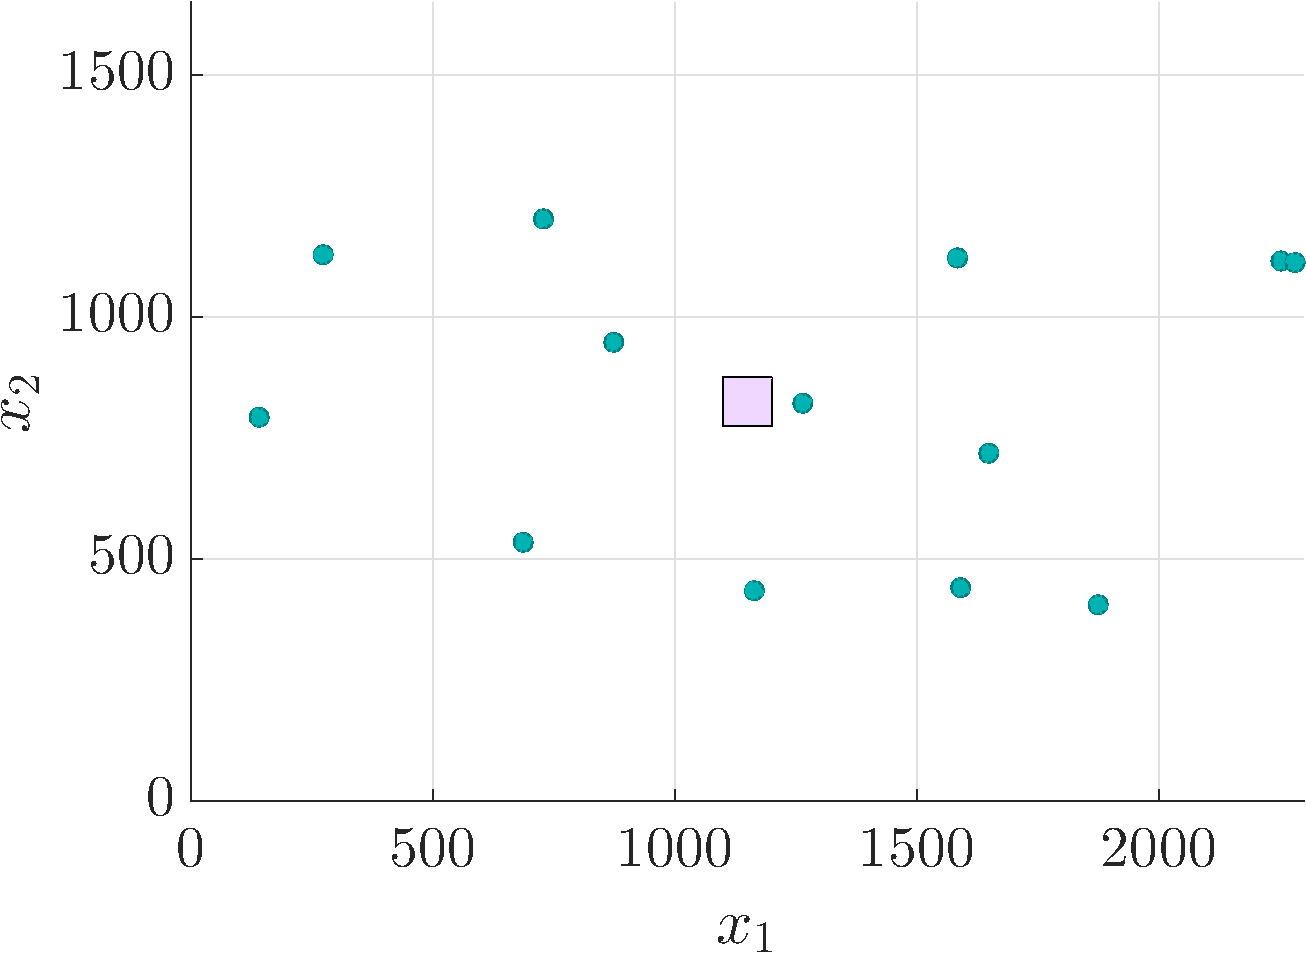
\includegraphics[width=0.4\textwidth]{series3D/setup_aerial_nolegend.pdf} \hfill
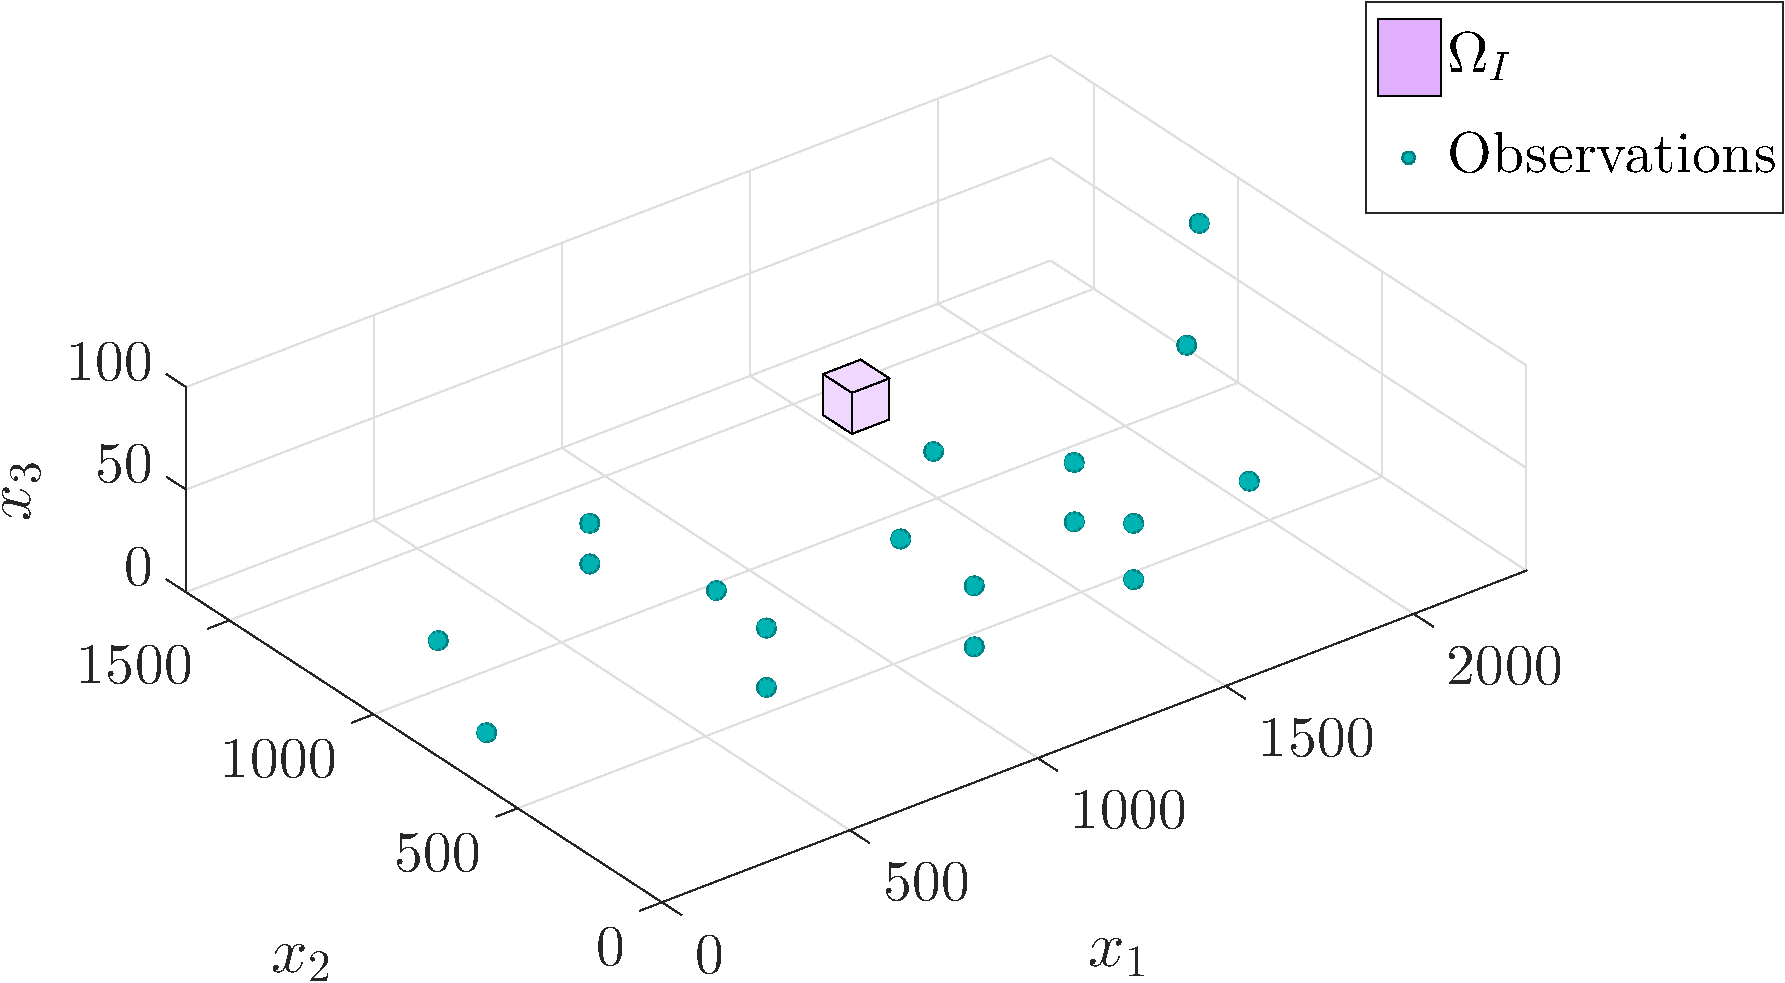
\includegraphics[width=0.55\textwidth]{series3D/setup_3view.pdf} \\ 
\vspace{\baselineskip}
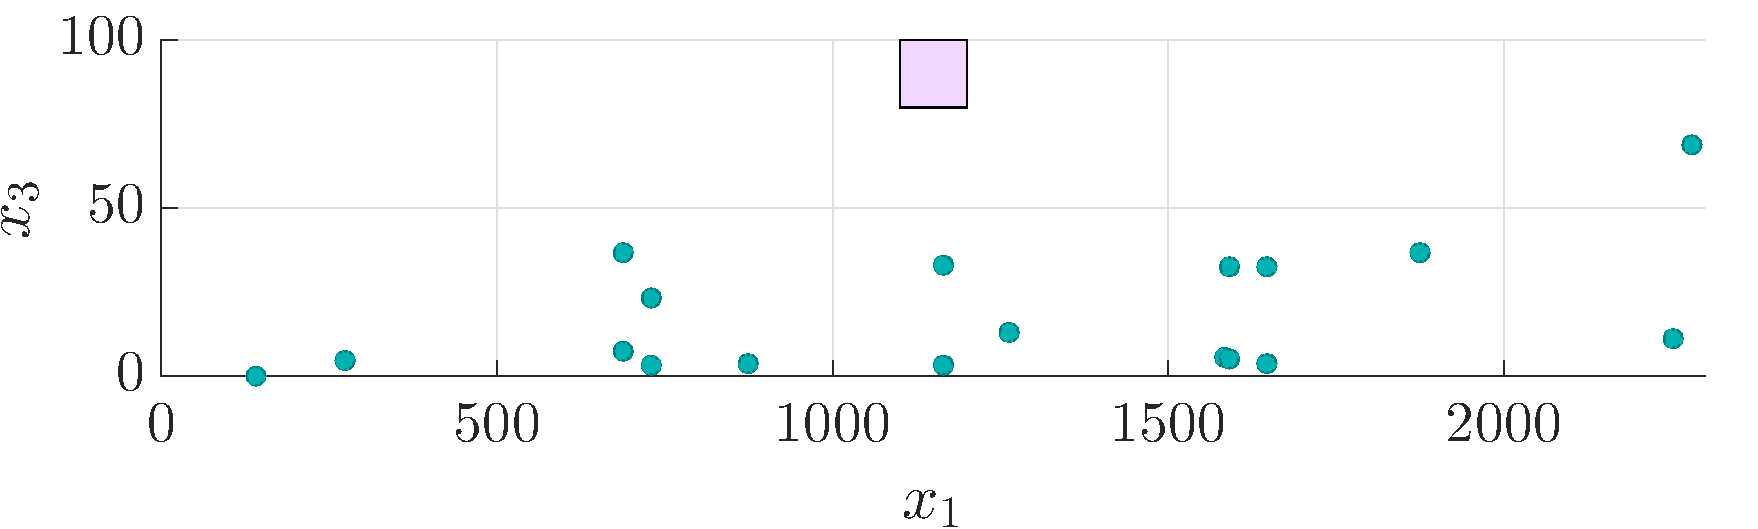
\includegraphics[width=0.6\textwidth]{series3D/setup_side_view.pdf}
\caption{Three views of the locations of the observations and the QoI region.}
\label{fig:setup3D}
\end{figure}
%
We continue to use the FEM with a continuous Galerkin formulation and Lagrange elements. The domain is discretized by a regular mesh of hexahedrons, with 25, 45, and 30 elements along the $x_1$, $x_2$, and $x_3$ directions, respectively; each variable has 37,076 degrees of freedom. The cell P\'{e}clet is small enough to not require stabilization.

%------------------------------------------------------------%
\subsubsection{Adaptive Model Refinement Results} \label{sec:ref3D}
%------------------------------------------------------------%

We now present the results of solving the inference problem using Algorithm~\ref{alg:refSeries}, with a relative error tolerance of $0.1\%$. At each iteration, we choose the $10\%$ of the basis functions with the largest error for model refinement; since each linear Lagrange basis function has eight elements in its support, the number of additional elements marked for refinement in each iteration may be larger. All simulations are run on a single processor. Table~\ref{tab:ref3D} shows the runtime and error at the end of each iteration. For the high-fidelity inverse problem, the Newton solver does not converge with a constant initial guess ($(p,u,z)=(0,5,0)$); instead, we solve the low-fidelity inverse problem and use its solution as the initial guess for the high-fidelity inverse problem. Each iteration of the adaptive algorithm uses the solution of the previous iteration as its initial guess. The runtime for each iteration of the adaptive algorithm is the total runtime, from the beginning of the adaptivity to the calculation of the error estimate for that iteration.
%
\begin{table}[h]
\centering
\begin{tabular}{c|c|c|c|c|c}
\multirow{2}{*}{Case} & \multirow{2}{*}{$\%$HF} & \multirow{2}{*}{QoI} & Relative Error & Relative Error & Total \\ 
& & & (Estimated) & (Actual) & Time (s) \\ \hline
LF   & 0    & 1068856 & -0.37511 & -0.48784 & 160 \\
MF01 & 16.7 & 577582  & -0.03831 & -0.05222 & 1110 \\
MF02 & 29.0 & 548904  & 0.00219  & -0.00272 & 1800 \\
MF03 & 42.3 & 547773  & 0.00032  & -0.00064 & 2220 \\
HF   & 100  & 547420  & 0        & 0        & 6210 \\
\end{tabular}
\caption{Runtime and relative errors of adaptive algorithm iterations given relative error tolerance of $0.001$ and $10\%$ of basis function marked for refinement per iteration.}
\label{tab:ref3D}
\end{table}
%
Compared to the previous examples in Section~\ref{sec:cdvcdr} with similar physics in the pair of models, we notice that in this case the estimated relative error in the later iterations is similar to the actual relative error in magnitude, but not in sign. This is likely due to the additional difference in the diffusive coefficient of the two models in this case. The sign difference does not, however, prevent the algorithm from finding a mixed-fidelity model for which the QoI matches the high-fidelity QoI to within $0.1\%$, but in about a third of the time. %what happens if you go on forever? the sign corrects itself in the next two iterations, and then becomes wrong again...also final all-HF QoI doesn't quite agree with invHF version (agrees to five sig figs)...also 'continuation' this way is faster (4600) than the other continuation schemes you tried...if we want to open this can of worms, will probably have to do more in-depth search of existing continuation algorithms...

The domain divisions for the three adaptive iterations are shown in Figure~\ref{fig:divvy3D}. We see that the error decomposition causes the first refinement iteration to target the QoI region and observations. Around the QoI region, the first iteration refines the domain completely in the $x_3$ direction, possibly reflecting the large difference in the high-fidelity dispersion tensor $D$ and the low-fidelity dispersion coefficient in the $x_3$ direction.
%
\begin{figure}[h]
\centering
\begin{subfigure}[t]{0.32\textwidth}
\centering
\includegraphics[width=\textwidth]{series3D/run_0p1/divvy1_whitebg_shiftaxes.png} 
\caption{MF$_1$}
\label{fig:ref3D_1}
\end{subfigure}
\begin{subfigure}[t]{0.32\textwidth}
\centering
\includegraphics[width=\textwidth]{series3D/run_0p1/divvy2_whitebg_shiftaxes.png} 
\caption{MF$_2$}
\end{subfigure}
\begin{subfigure}[t]{0.32\textwidth}
\centering
\includegraphics[width=\textwidth]{series3D/run_0p1/divvy3_whitebg_shiftaxes.png} 
\caption{MF$_3$}
\end{subfigure}
\caption{Domain division for mixed-fidelity models (low-fidelity convection-diffusion model used in pink portion, high-fidelity convection-diffusion-reaction model used in blue portion).}
\label{fig:divvy3D}
\end{figure} 
%
The amount of time required by the adaptive algorithm of course depends on the chosen error tolerance as well as the amount of additional model refinement between successive iterations. Refining a larger region per iteration runs the risks of refining in the wrong areas due to linearization about a $\Psi_{MF}$ that is very different from $\Psi_{HF}$, but can also allow one to reach the chosen error tolerance in fewer iterations and less runtime. We compare the runtimes for a more conservative choice of refinement rate; given the same error tolerance, we instead choose the $5\%$ of the basis functions with the largest error for model refinement. Table~\ref{tab:ref3D_dainty} shows the runtime and error at the end of each of these iterations, and Figure~\ref{fig:divvy3D_dainty} shows the domain divisions for the six corresponding mixed-fidelity models.
%
\begin{table}
\centering
\begin{tabular}{c|c|c|c|c|c}
\multirow{2}{*}{Case} & \multirow{2}{*}{$\%$HF} & \multirow{2}{*}{QoI} & Relative Error & Relative Error & Total \\ 
& & & (Estimated) & (Actual) & Time (s) \\ \hline
LF   & 0    & 1068856 & -0.37511 & -0.48784 & 160 \\
MF01 & 9.27 & 613419  & -0.06649 & -0.10759 & 1040 \\
MF02 & 16.9 & 558523  & 0.00208  & -0.01988 & 1860 \\
MF03 & 23.7 & 550323  & 0.00456  & -0.00528 & 2420 \\
MF04 & 30.4 & 548225  & 0.00302  & -0.00147 & 2970 \\
MF05 & 37.2 & 547744  & 0.00120  & -0.00059 & 3309 \\
MF06 & 44.6 & 547532  & 0.00035  & -0.00020 & 3642 \\
HF   & 100  & 547420  & 0        & 0        & 6210 \\
\end{tabular}
\caption{Runtime and relative errors of adaptive algorithm iterations given relative error tolerance of $0.001$ and $5\%$ of basis function marked for refinement per iteration.}
\label{tab:ref3D_dainty}
\end{table}
%
\begin{figure}[h]
\centering
\begin{subfigure}[t]{0.32\textwidth}
\centering
\includegraphics[width=\textwidth]{series3D/run_0p05/divvy1_whitebg_shiftaxes.png} 
\caption{MF$_1$}
\label{fig:ref3d_dainty1}
\end{subfigure}
\begin{subfigure}[t]{0.32\textwidth}
\centering
\includegraphics[width=\textwidth]{series3D/run_0p05/divvy2_whitebg_shiftaxes.png} 
\caption{MF$_2$}
\label{fig:ref3d_dainty2}
\end{subfigure}
\begin{subfigure}[t]{0.32\textwidth}
\centering
\includegraphics[width=\textwidth]{series3D/run_0p05/divvy3_whitebg_shiftaxes.png} 
\caption{MF$_3$}
\end{subfigure}
\begin{subfigure}[t]{0.32\textwidth}
\centering
\includegraphics[width=\textwidth]{series3D/run_0p05/divvy4_whitebg_shiftaxes.png} 
\caption{MF$_4$}
\end{subfigure}
\begin{subfigure}[t]{0.32\textwidth}
\centering
\includegraphics[width=\textwidth]{series3D/run_0p05/divvy5_whitebg_shiftaxes.png} 
\caption{MF$_5$}
\end{subfigure}
\begin{subfigure}[t]{0.32\textwidth}
\centering
\includegraphics[width=\textwidth]{series3D/run_0p05/divvy6_whitebg_shiftaxes.png} 
\caption{MF$_6$}
\end{subfigure}
\caption{Domain division for mixed-fidelity models (low-fidelity convection-diffusion model used in pink portion, high-fidelity convection-diffusion-reaction model used in blue portion).}
\label{fig:divvy3D_dainty}
\end{figure} 
%
We again observe that the estimated relative error in the later iterations is similar to the actual relative error in magnitude, but not in sign. It can also be seen in Figure~\ref{fig:ref3d_dainty1} that the largest error first comes from the QoI region and area below it, and the observations. Similarly to the examples in Section~\ref{sec:cdvcdr}, of the observations, refinement is least necessary around the ones furthest downstream of the QoI region.

We see that although the more conservative refinement rate requires more iterations and runtime to reach the desired error tolerance, the adaptive algorithm requires about a half of the time of the high-fidelity inverse problem. We note that, although both refinement rates result in similar final refinement proportions for our chosen error tolerance ($42.4\%$ versus $44.6\%$), they do not necessarily produce the same refined regions (compare Figures~\ref{fig:ref3D_1} and \ref{fig:ref3d_dainty2}) or relative error for a given refinement proportion. A slower refinement rate also does not necessarily produce a smaller (estimated or true) relative error, or a more accurate relative error estimate, for a given refinement proportion.

